\documentclass{article}
\usepackage{iclr2026_conference,times}
\input{math_commands.tex}

\usepackage{hyperref}
\usepackage{url}
\usepackage{booktabs}
\usepackage{xcolor}
\usepackage{colortbl}
\usepackage{multirow}
\usepackage{graphicx}
\usepackage{tikz}
\usepackage{pgfplots}
\pgfplotsset{compat=1.18}
\usepackage{algorithm}
\usepackage{algpseudocode}
\usepackage{enumitem}
\usepackage{amsmath,amssymb,amsthm}
\newtheorem{proposition}{Proposition}
\newtheorem{remark}{Remark}
\newtheorem{definition}{Definition}

\title{Active Forgetting: \\ A Missing Memory Primitive for LLM Agents}

\author{Anonymous Authors}

\newcommand{\fix}{\marginpar{FIX}}
\newcommand{\new}{\marginpar{NEW}}

%\iclrfinalcopy

\begin{document}

\maketitle

% =====================================================
% ABSTRACT — paper-writing skill V2: Challenge -> Insight -> Contribution
% =====================================================
\begin{abstract}
LLM agent memory systems---KV cache compression~\citep{zhang2023h2o,xiao2024streamingllm,li2024snapkv}, hierarchical memories~\citep{packer2023memgpt,li2025memos,park2023generative}, summarization-based long-term memory~\citep{wu2023recursivesumm}---decide what to retain by score (importance, recency, attention salience, semantic similarity), agnostic to who produced the content and under what evidence subset. We argue this is a category error. LLM-generated content is \emph{provisional}: produced under a partial subset of the eventual evidence and not retracted when later evidence refines it. Persisting provisional content under the same role as externally observed evidence biases subsequent decisions, in direct analog to source-monitoring failures in human cognition~\citep{johnson1993source}. We identify \emph{active forgetting}---content-typed eviction at decision time, conditioned on epistemic provenance rather than score---as a missing memory primitive, distinct from generation and retention. Three lines of evidence show forgetting is structurally necessary, not a deployment optimization. (i) On Lost-in-Conversation with Qwen2.5-14B, dropping all prior assistant tokens at every turn (\textsc{Fresh-Every}) reaches 103\% gap recovery and exceeds the single-turn ceiling; the dose-response is a cliff (4--23\% recovery for any 25--75\% retention vs.\ 87\% for full removal), and Proposition~\ref{prop:cliff} shows any non-empty subset of provisional content perpetuates contamination. (ii) The mechanism is attention-mediated rather than format-mediated: prior assistant commitments receive per-token attention comparable to the system prompt while \texttt{[OUTDATED]} markers leave accuracy at the Sharded floor---content typing must be structural, not textual. (iii) Uniform forgetting fails when some content is verified state: on BFCL v4 stateful tool use, \textsc{Fresh-Every} collapses from 0.875 to 0.090 while typed \textsc{CacheGuard} (drops provisional claims, retains tool results) matches the strongest baseline (0.280 vs.\ 0.295, $p{=}0.66$). The effect replicates across five models in four architecture families. We chart a forgetting-operation taxonomy (attention-zero, sentence drop, turn drop, typed-block drop) and introduce VCHR and HCHR alongside PCHR to make forgetting measurable. Implications cut across the stack: KV-compression heuristics that retain attention-important tokens preferentially preserve harmful anchors; agentic memory frameworks that summarize history inherit the contamination; chat protocols need forgetting as a first-class primitive alongside generation and retention.
\end{abstract}

% =====================================================
% 1 INTRODUCTION — V3 (general-to-specific) + V4 (observation-driven)
% =====================================================
\section{Introduction}

% --- Para 1: A category error in LLM agent memory ---
The dominant abstraction for LLM agent memory decides retention by score---attention salience in KV cache compression~\citep{kwon2023vllm,zheng2024sglang,liu2025lmcache,zhang2023h2o,xiao2024streamingllm,li2024snapkv}, importance-recency-relevance in hierarchical memory~\citep{packer2023memgpt,li2025memos,park2023generative,memagent2026}, semantic similarity in retrieval-augmented memory, position in summarization-based memory~\citep{wu2023recursivesumm}. None condition retention on \emph{who produced the content and under what evidence}. This is the question that distinguishes externally observed data (a user statement, a successful tool call) from LLM-generated inference (an assistant response, a CoT step, a summary-of-summaries) under partial information. Cognitive psychology calls the analogous human capacity \emph{source monitoring}~\citep{johnson1993source}; its failure---attributing internally generated content to external observation---produces systematic recall errors. We argue current LLM memory architectures bake the same failure in by design: stored inference is rendered identically to stored evidence, and downstream generation conditions on both as if both were authoritative. We name the missing operation \emph{active forgetting}: content-typed eviction at decision time, conditioned on epistemic provenance rather than score, complementing generation and retention. Where retention answers ``can this prefix be reused?'', forgetting answers ``should this content remain eligible for future decisions?''. Existing serving systems are intentionally agnostic to the latter; we show this is not a benign optimization but a correctness-bearing omission.

% --- Para 2: Multi-turn conversations mix evidence and commitment ---
A multi-turn agent context is not a static document. A user message is external evidence. A successful tool observation is external evidence. But an assistant response is a model action---often a provisional commitment made under partial information---which the standard chat protocol then serializes into the next prompt as if it were evidence. Recent work~\citep{laban2025lost} reports that multi-turn LLM accuracy on underspecified conversations drops 30--40\% relative to single-turn fully-specified versions, even though by conversation's end the assistant has received the same information. Existing remedies---prompt evolution~\citep{agrawal2025gepa}, harness search~\citep{lee2026metaharness, zhang2024aflow}, dialogue policy learning~\citep{chen2024act}, and the LiC paper's own \textsc{Recap}---all retain the assistant's prior responses in context. \textsc{Recap} attains the highest message-level prefix-cacheability proxy (mPCHR 0.851 in our measurement) yet recovers only 65\% of the multi-turn gap, 22\,pp below \textsc{Fresh-Last}. Optimizing for cacheability has a hidden cost.

% --- Para 3: Observation: cache reuse and validity are not the same property ---
We observe that the LLM's prior responses, generated under partial information when the user has not yet revealed all shards, are systematically wrong but stored in context with identical chat-template formatting as user evidence. They are physically reusable (every prefix-cache lookup retrieves them) but epistemically invalid (the conversation's later user shards now contradict them). We propose the distinction: \emph{can reuse $\neq$ should reuse}. To make this operational, we introduce two metrics alongside PCHR. \textbf{VCHR} (valid cache hit rate) is the fraction of reused tokens belonging to blocks that remain epistemically valid evidence under the current state. \textbf{HCHR} (harmful cache hit rate) is the fraction of reused tokens whose presence counterfactually flips the answer from correct to wrong.

% --- Para 4: Decisive empirical patterns + four counter-intuitive findings ---
On Lost-in-Conversation with Qwen2.5-14B, the standard \textsc{Sharded} protocol (no forgetting) attains mPCHR 0.751 but accuracy 0.208. \textsc{Recap}, which re-states user information but does not forget assistant outputs, attains the highest mPCHR (0.851) and accuracy 0.625. A five-line forgetting policy that drops all prior assistant tokens at every turn (\textsc{Fresh-Every}) attains mPCHR 1.000, VCHR 1.000, and accuracy 0.875. The 22\,pp gap between \textsc{Recap} and \textsc{Fresh-Last} (65\% vs 87\% recovery, $\Delta{=}+0.146$) isolates to the single line distinguishing them: whether the prior assistant trace is forgotten at decision time. Four findings sharpen this picture. \emph{Cliff, not gradient.} Dropping any 25--75\% of prior assistant messages recovers only 4--23\% of the gap, while complete removal at $K{=}1.0$ recovers 87\%---no partial compromise works (Figure~\ref{fig:dose-curve}). \emph{Capability inversion.} Qwen2.5-7B under \textsc{Fresh-Last} reaches 0.917, nominally above 14B \textsc{Fresh-Last} (0.771) and the 14B Concat ceiling (0.854); larger models generate more coherent commitments under partial information, producing stronger anchors rather than resistance. The nominal exceedance is partially attributable to multi-attempt advantage on Qwen-7B (Appendix~\ref{app:bestofN}), but on Llama-3.1-8B the same ordering survives a best-of-$N$ control. \emph{Attention, not format.} Marking prior messages with \texttt{[OUTDATED PARTIAL-INFO COMMITMENT]} yields 0.307, barely above the 0.208 baseline and far below \textsc{Fresh-Last} (0.771); text markers do not override attention-mediated anchoring, confirming that the conflict is architectural rather than instructional. \emph{Task-structure dependent.} \textsc{Recap} recovers 86\% of the gap on tool-use actions but only 27\% on code generation (Table~\ref{tab:main}); single-call commitments are easier to partially override than multi-step ones.

% --- Para 5: From observation to framework ---
We synthesize these findings into \textsc{CacheGuard}, a typed forgetting controller. It (i) classifies each context block by epistemic role---system instruction, user evidence, tool result, assistant artifact, assistant claim, assistant plan; (ii) applies an eligibility rule that retains user/tool blocks but forgets provisional assistant claims; and (iii) renders a stable-valid prefix plus a volatile suffix at LLM-call time. \textsc{CacheGuard} is deployable client-side with no training, no model change, and no proprietary serving access.

% --- Para 6: Contributions summary (4 items) ---
Our contributions are four. \emph{First}, we identify \emph{active forgetting of provisional content} as a missing memory primitive in LLM agent design, distinct from generation and retention. Existing serving and memory systems---KV-cache compressors, hierarchical memories such as MemGPT, summarization-based long-term memory---decide retention by score (attention salience, importance, recency, semantic similarity), agnostic to who produced the content and under what evidence. This is a category error rather than an optimization gap, with the same structure as the source-monitoring failure that produces internal-vs-external misattributions in human cognition~\citep{johnson1993source}. \emph{Second}, we formalize the cliff: Definition~\ref{def:provisional} characterizes provisional content as anything produced by a generator $\pi(\cdot \mid \mathcal{E}_<)$ conditioned on a strict subset of the eventual evidence, and Proposition~\ref{prop:cliff} shows that any non-empty retained subset perpetuates posterior contamination. The dose-response cliff at $K{=}1.0$ (Figure~\ref{fig:dose-curve}), the marked-history null (textual \texttt{[OUTDATED]} markers leave accuracy at the floor), and the universal failure of attention-salience compression all follow as corollaries. A concrete instance is the GSM8K/651 case (Appendix~\ref{app:anchor-id}): the model's Turn-1 commitment ``we need specific data regarding her sales'' anchors every subsequent response to a meta-stance of restating-the-steps; removing that single sentence flips the final-turn answer from 0 to 1, even though the surrounding eight turns and the gold value are unchanged. \emph{Third}, we instantiate the primitive as a deployable controller. \textsc{CacheGuard} parses each context block by epistemic role and applies a typed eligibility rule that retains authoritative content while evicting provisional commitments, requiring no retraining and shipping client-side; PCHR, VCHR, and HCHR are three measurement metrics that make the abstract claim quantifiable alongside the standard prefix-cache statistic. \emph{Fourth}, we validate empirically. On Lost-in-Conversation, \textsc{Fresh-Every} recovers 103\% of the multi-turn gap and exceeds the same-model single-turn ceiling; the cliff, the marked-history null, and the attention-mediation signature replicate across five models in four architecture families (Qwen-7B/14B, Llama-3.1-8B, Mistral-7B, Gemma-2-9B). On BFCL v4 stateful tool use, uniform forgetting collapses to 0.090 while \textsc{CacheGuard} matches the strongest baseline at 0.280 ($p{=}0.66$, ns)---direct evidence that the operator must be content-typed, not uniform.

% =====================================================
% 2 RELATED WORK
% =====================================================
\section{Related Work}

\paragraph{Multi-turn LLM degradation and mitigation.}
\citet{laban2025lost} document the multi-turn underspecified failure mode and propose \textsc{Recap} and \textsc{Snowball}, which re-state user information but retain prior assistant responses, recovering 30--52\% of the gap. The same study shows that reasoning models (o3, DeepSeek-R1) degrade similarly: extra test-time compute does not, on its own, help models strategize across turns. \citet{weston2025multichallenge} corroborate this on MultiChallenge, where all frontier models score under 50\% on instruction retention and self-coherence. \citet{li2026intent} propose a Mediator-Assistant architecture that rewrites user inputs while again preserving assistant history. Harness and prompt search systems~\citep{lee2026metaharness,zhang2024aflow,agrawal2025gepa} optimize scaffolding or prompt text but operate within a fixed context-retention protocol. The dialogue-systems community addressed multi-turn state maintenance via explicit slot-filling~\citep{wu2019transferable}; our finding shows that implicit state tracking through LLM history retention is insufficient, and selective forgetting of agent commitments outperforms retention on knowledge-intensive tasks. Our diagnosis shows that a protocol-level change dominates all prompt-level interventions on LiC.

\paragraph{Closest concurrent work: assistant-history filtering.}
\citet{huang2026benefit} report that omitting prior assistant responses preserves quality and reduces context up to 10$\times$ on in-the-wild conversations, identifying ``context pollution'' on 36.4\% of self-contained turns. Our work extends that finding along four axes that together turn an empirical observation into a primitive. We construct a controlled sharded benchmark where the failure is reproducible by design (rather than relying on in-the-wild prevalence); we identify a binary-cliff mechanism (Figure~\ref{fig:dose-curve}) showing that partial filtering does not work even at 50\% retention, with a one-sentence worked example (GSM8K/651 in Section~\ref{sec:selective-drop}) demonstrating the cliff at the granularity of a single retained commitment; we formalize the phenomenon as a \emph{cache-validity} problem with three metrics (PCHR, VCHR, HCHR) that plug into the serving stack; and we ship \textsc{CacheGuard}, a typed reuse layer that handles the stateful-tool reversal (Section~\ref{sec:bfcl}) where uniform assistant-history deletion is harmful. Three concurrent papers identify the same anchoring phenomenon under different names. \citet{wang2025proactive} introduce PI-LLM and show log-linear decay in retrieval accuracy under proactive interference even when the target value is adjacent to the query; their key result---``ignore earlier inputs'' instructions fail---directly corroborates our marked-history null. \citet{li2026inertia} call the effect ``conversational inertia'' and propose periodic blind context clipping; \citet{zhang2026rlanchor} address it via expensive RL fine-tuning; and \citet{xu2026sleepgate} build a learned sleep-cycle gate inside the KV cache. Each of these accepts the phenomenon and proposes a remedy on the wrong axis: position-based clipping, learned-importance retention, or weight-level training. None give a regime-independent theorem, a content-type criterion, or a deployable training-free controller that handles both the stateless-reasoning and stateful-tool regimes within a single design.

\paragraph{Memory architectures and the axis of typing.}
Existing LLM memory systems either treat all stored content homogeneously or distinguish it on axes orthogonal to epistemic provenance. KV-cache compression~\citep{zhang2023h2o,xiao2024streamingllm,li2024snapkv} and most retrieval-augmented memories evict by score and are blind to who produced a token. Hierarchical memories~\citep{packer2023memgpt,li2025memos,memagent2026} record metadata---MemOS in particular logs an origin signature (user/inference/external/finetuning)---but use it for audit, not for governance: scheduling and eviction remain score-based. Generative Agents~\citep{park2023generative} structurally separates observations, plans, and reflections, yet the design decision is to \emph{elevate} reflections (synthetic syntheses) via importance scoring---the opposite axis from ours, which would evict them as provisional. Reflexion~\citep{shinn2023reflexion} maintains a reflection buffer that grows monotonically and is treated as positive signal. ReadAgent~\citep{lee2024readagent} keeps original text as a fallback to gist memories but motivates the redundancy as compression efficiency, not as a hedge against gist-level provisionality. The closest engineering analogs to our intervention are \citet{li2026inertia}'s position-based context clipping for conversational inertia and \citet{activecontextcuration2026}'s RL-trained context curator that selects ``reasoning anchors''; both keep the question on the wrong axis (recency, learned importance), neither defines a content-type criterion. Our contribution is to make epistemic provenance a first-class typing axis and to formalize when a typed evictor is necessary: the contamination cliff (Proposition~\ref{prop:cliff}) is a regime-independent prediction, in direct analog to source monitoring~\citep{johnson1993source} in human cognition. We distinguish active forgetting at \emph{inference time} on the KV cache from machine unlearning, which operates on \emph{training-time weights}; these address categorically different failure modes. Anchoring bias~\citep{tversky1974anchoring} and ACT-R activation decay~\citep{anderson1998actrarch} provide behavioral and architectural antecedents but neither identifies provenance as the typing axis. \citet{khattab2025contexteng} survey context engineering; \citet{ace2025} name a related ``context collapse'' phenomenon across agentic, RAG, and summarization regimes and propose a systems-level evolution mechanism. Both leave open the typed-eviction primitive that our work makes explicit.

\paragraph{KV cache systems, position bias, and compression.}
\citet{kwon2023vllm}, \citet{zheng2024sglang}, and \citet{liu2025lmcache} optimize physical cache hit rate. \citet{zhang2023h2o,xiao2024streamingllm,li2024snapkv} compress the KV cache by attention salience. All treat reusable as reuse-worthy and select tokens to retain. The over-attended tokens in our setting are content-anchored prior assistant commitments, distinguishing them from position-zero attention sinks~\citep{xiao2024streamingllm,sun2025attentionsink} and from the U-shaped position bias of \citet{liu2023lostmiddle}. The cliff dose-response (Section~\ref{sec:selective-drop}) rules out salience-based compression as a fix---any retention heuristic that keeps a non-trivial fraction of prior assistant tokens fails. \citet{contextualdrag2026} document a related token-level anchoring effect; we quantify it through cache-validity metrics and provide a deployable forgetting policy. Recursive summarization~\citep{wu2023recursivesumm} compresses but retains assistant-generated content, which our marked-history null predicts will inherit the anchoring effect.

\paragraph{Sentence-level anchoring and causal attribution.}
\citet{thoughtanchors2025} identify ``thought anchors'' within chain-of-thought reasoning: individual sentences whose removal flips a wrong-to-correct prediction, finding a small fraction ($\sim$5\%) of CoT sentences carry disproportionate causal weight. Their scope is \emph{intra-turn}---sentences within a single response. Our finding identifies the analogous phenomenon \emph{cross-turn}: entire prior assistant responses from earlier conversation turns act as anchors on the final response, via the same attention-mediated mechanism (Section~\ref{sec:attention-probe}). Both are causal (removal flips outcome) and localizable via ablation; Appendix~\ref{app:anchor-id} extends their sentence-level methodology to cross-turn assistant history. \citet{aipsychosis2026} show that LLMs in extended agentic conversations develop ``AI psychosis''---persistent incorrect beliefs resisting correction under explicit counter-evidence---consistent with our contamination framing and the Marked-History null. Causal attribution methods~\citep{gradienttracing2025} trace output causation to input tokens; HCHR operationalizes the same question at the block level, connecting it to the serving-layer design of Section~\ref{sec:cacheguard}.

% =====================================================
% 3 BACKGROUND
% =====================================================
\section{Background and Problem Setting}
\label{sec:background}

\paragraph{Sharded multi-turn underspecification.}
We use the Lost-in-Conversation \emph{sharded} benchmark~\citep{laban2025lost}, which transforms a single-turn fully-specified instruction into a sequence of $K$ \emph{shards}---atomic information units, each revealed in a separate user turn. Across $K$ turns, the user simulator reveals one shard per turn until all are revealed. The assistant produces a response after each user turn. The conversation terminates either when an automatic verifier judges an assistant response as a correct answer attempt, or when all shards have been revealed. We evaluate on the LiC \texttt{multi\_heldout} split covering three task families with non-trivial Concat ceilings: math (GSM8K), code (HumanEval / LiveCodeBench), and tool-use (BFCL actions).

\paragraph{Reference protocols.}
LiC defines two reference protocols. \textsc{Concat} concatenates all shards in a single user message and queries the LLM once; this is the single-turn ceiling. \textsc{Sharded} runs the protocol described above and is the floor. The gap between these defines the multi-turn drop. LiC also reports two mitigations: \textsc{Snowball} re-states all prior shards at each turn (keeps full history), and \textsc{Recap} appends a final user message summarizing all revealed shards (also keeps full history). Both partially close the gap.

% =====================================================
% 4 METHOD
% =====================================================
\section{Method}
\label{sec:method}

\subsection{Three cache metrics for multi-turn LLM serving}
\label{sec:metrics}
Standard serving systems report \emph{physical cache hit rate}:
\begin{equation}
\text{PCHR} = \frac{\text{reused prefix tokens}}{\text{queried prompt tokens}}.
\end{equation}
We complement it with two metrics that depend on the conversation's evolving epistemic state. Let $\mathcal{B}$ be the set of context blocks reused at decision time, and let $\text{valid}(b, s)$ denote whether block $b$ is still epistemically valid evidence under current state $s$ (Section~\ref{sec:eligibility}).
\begin{equation}
\text{VCHR} = \frac{\sum_{b \in \mathcal{B}} \mathbf{1}[\text{valid}(b, s)] \cdot |b|}{\sum_{b \in \mathcal{B}} |b|}.
\end{equation}
\begin{equation}
\text{HCHR} = \frac{\sum_{b \in \mathcal{B}} \mathbf{1}[\text{flips}(b)] \cdot |b|}{\sum_{b \in \mathcal{B}} |b|},
\end{equation}
where $\text{flips}(b)$ is 1 iff removing $b$ counterfactually changes the outcome from incorrect to correct. PCHR alone defines the standard objective; an ideal serving stack maximizes $\text{PCHR} \times \text{VCHR}$ while minimizing HCHR. Existing systems measure only PCHR; multi-turn agentic deployments require also tracking VCHR and HCHR.

\subsection{A taxonomy of forgetting operations}
\label{sec:taxonomy}
Forgetting can act at five granularities, each with a different domain of validity. Table~\ref{tab:forget-taxonomy} summarizes; the protocols evaluated in this paper (Section~\ref{sec:main-protocol}) instantiate four of the five rows.

\begin{table}[h]
\centering
\caption{Forgetting-operation taxonomy. Each operator differs in what it removes from the LLM's effective context. Coarser operators are simpler but lose authoritative content; finer operators need a typing signal.}
\label{tab:forget-taxonomy}
\small
\setlength{\tabcolsep}{4pt}
\begin{tabular}{p{0.17\linewidth}p{0.36\linewidth}p{0.39\linewidth}}
\toprule
Granularity & Operator & Domain of validity \\
\midrule
Token-attention & Zero attention to a token set (no deletion) & Cases where eviction would break cache structure (S8b). \\
Sentence & Drop specific sentences within a turn & Intra-turn CoT~\citep{thoughtanchors2025}; cross-turn in App.~\ref{app:anchor-id}. \\
Turn-uniform & Drop all prior assistant turns (Fresh-Last / Fresh-Every) & Stateless reasoning where every assistant turn is provisional. Fails when some assistant content carries verified state. \\
Block-typed & Drop provisional, retain authoritative (CacheGuard) & Mixed regimes (BFCL v4: tool calls and results are authoritative; asst-text is provisional). \\
Conversation-reset & Rebuild context per query (Concat) & Bounded single-shot; loses history. \\
\bottomrule
\end{tabular}
\end{table}

\subsection{Protocol variants}
All protocols differ only in which subset of $\{a_1, \ldots, a_{t-1}\}$ is passed to the LLM at turn $t$. \textsc{Sharded}: full history $[s, u_1, a_1, \ldots, u_t]$. \textsc{Fresh-Last}: at the final turn, pass $[s, u_{\text{concat}}]$ dropping all prior assistant messages (five lines of code). \textsc{Fresh-Every}: at every turn $t$, pass $[s, u_{\text{concat-so-far}}]$; the LLM never sees its own prior responses. \textsc{Marked-History}: retain all prior assistant messages but prefix each with \texttt{[OUTDATED PARTIAL-INFO COMMITMENT]}, testing whether anchoring is format-confusion (H3) or attention-mediated (H1). \textsc{Selective-Drop}: parametrized by $K \in [0,1]$, drops the first (or last) $K$ fraction of prior assistant messages; $K=0$ is \textsc{Sharded}, $K=1$ is \textsc{Fresh-Last}. These cover the turn-level uniform and block-typed rows of Table~\ref{tab:forget-taxonomy}; sentence-level (Appendix~\ref{app:anchor-id}) and token-attention-level (Section~\ref{sec:limitations}) are evaluated separately.

\subsection{CacheGuard: validity-aware reuse}
\label{sec:cacheguard}

The protocols above reveal a Pareto problem: \textsc{Sharded} and \textsc{Recap} have high mPCHR but low VCHR; \textsc{Fresh-Every} has high VCHR but its full-context-rebuild approach forfeits potential cache reuse on a stable system+constraint prefix. A practical serving layer would combine high PCHR (cacheable stable prefix) with high VCHR (no provisional commitments retained). This is what \textsc{CacheGuard} provides.

\paragraph{Block Parser.}
\label{sec:eligibility}
We type each non-log message in the conversation. The authoritative types are \texttt{system} (the protocol instruction; always valid), \texttt{user\_evidence} (a user-revealed shard; always valid), and \texttt{tool\_observation} (a successful tool result; always valid). The assistant-side types are \texttt{assistant\_artifact} (a code block, table, or named output produced by the assistant), \texttt{assistant\_claim} (an answer attempt or boxed/bracketed final answer), \texttt{assistant\_clarification} (a question to the user), and \texttt{assistant\_plan} (intended next steps without producing an artifact). Two cross-block relations are also tracked: \texttt{contradicted\_by} (a block invalidated by a later block) and \texttt{referenced\_by} (artifacts subsequently referenced by user or tool blocks).

\paragraph{Eligibility Controller.}
A block $b$ is reuse-eligible exactly when it is a system / user / successful-tool block, or an artifact that is later referenced by user or tool blocks, or a clarification (asking rather than committing). Provisional claims and plans are excluded by default; any block marked \texttt{contradicted\_by} a later block is also excluded.

\paragraph{Renderer.}
At LLM-call time, the rendered context is
\[
[\,\underbrace{s\;\Vert\;\textit{verified user constraints}\;\Vert\;\textit{verified tool state}}_{\text{stable valid prefix}}\;\Vert\;\underbrace{\textit{current turn}\;\Vert\;\textit{referenced artifacts}}_{\text{volatile suffix}}\,].
\]
The stable valid prefix is monotone-growing (only appended-to as new verified evidence arrives), maximizing PCHR; the volatile suffix is small and changes per turn. Provisional commitments live in a hidden side-buffer that the renderer does not pass to the LLM.

\paragraph{Renderer detail: user-shard consolidation.}
The renderer concatenates verified user shards into a single block in the stable prefix, rather than preserving multiple user-role messages. This is consistent with the typed-eligibility view---the user's accumulated evidence is a single epistemic unit---and matches how the task's underlying single-turn evaluator (\texttt{populate\_concat\_prompt}) presents the same content. On LiC the consolidation is exact (each shard contributes one bullet); on BFCL where the user's turn structure conveys timing, we keep user messages atomic. The choice is part of the typed renderer, not a benchmark hack.

% =====================================================
% 5 EXPERIMENTS
% =====================================================
\section{Experiments}
\label{sec:experiments}

\subsection{Setup}
We use Qwen2.5-14B-Instruct as the assistant model and Qwen2.5-7B-Instruct as the user simulator and grader. We evaluate on the LiC \texttt{multi\_heldout} split: 8 task instances per class across 3 task classes (math, code, actions) for 24 instances, each run with $N=2$ independent simulations. Per-class accuracy is computed by averaging per-instance accuracy (treating null/no-answer outcomes as failures), then averaging across instances within each class. The gap is measured as Concat$-$Sharded; gap recovery for a method $M$ is $(M - \text{Sharded}) / (\text{Concat} - \text{Sharded})$.

\subsection{Main result: protocol comparison}
\label{sec:main-protocol}

Table~\ref{tab:main} reports per-class accuracy and gap recovery. \textbf{Fresh-Last recovers 87\% of the gap, 22\,pp above LiC's Recap baseline (65\%). Fresh-Every recovers 103\%, exceeding the single-turn ceiling on average.}

\begin{table}[t]
\centering
\caption{Per-class accuracy and gap recovery on LiC \texttt{multi\_heldout} (Qwen2.5-14B). Sharded is the multi-turn floor; Concat is the single-turn ceiling. Gap recovery $= (\text{acc} - \text{Sharded}) / (\text{Concat} - \text{Sharded})$ averaged across the three classes.}
\label{tab:main}
\begin{tabular}{lcccc}
\toprule
Protocol & Math & Code & Actions & Gap recovered \\
\midrule
Sharded (floor) & 0.500 & 0.000 & 0.125 & 0\% \\
Concat (ceiling) & 0.938 & 0.625 & 1.000 & 100\% \\
\midrule
Recap~\citep{laban2025lost} & 0.833 & 0.167 & 0.875 & 65\% \\
\textbf{Fresh-Last (ours)} & 0.875 & 0.438 & 1.000 & \textbf{87\%} \\
\textbf{Fresh-Every (ours)} & 0.938 & 0.688 & 1.000 & \textbf{103\%} \\
\bottomrule
\end{tabular}
\end{table}

\subsection{Mechanism: anchoring is a cliff-dominated dose-response}
\label{sec:selective-drop}

We map the dose-response curve of partial history dropping by sweeping two complementary protocols: \textsc{Selective-Drop} drops the EARLIEST $K$ fraction of prior assistant messages, and \textsc{Drop-Latest} drops the LATEST $K$ fraction (Table~\ref{tab:dose}). Three observations emerge.

First, neither curve is a smooth concave dose-response. Dropping any partial fraction (0.25 to 0.75) yields gap recovery between 4\% and 23\%, far short of the full removal at $K=1.0$ which recovers 87\%. The cliff at $K=1.0$ is the dominant feature.

Second, the EARLIEST-vs-LATEST asymmetry is small but consistent: at $K=0.5$, both yield 0.235 vs 0.242; at $K=0.75$, EARLIEST yields 0.333 while LATEST yields 0.278. Removing earliest commitments is slightly more effective, supporting a weak ``earliest-as-root-anchor'' interpretation. But the magnitude is small ($\approx$5\,pp), and even at $K=0.75$, retained later commits still anchor downstream---no partial removal escapes the chain.

Third, the implication is sharper than a graded dose-response: \emph{any} retained partial-info commitment dominates attention at decision time, regardless of position. Interventions that keep ``most recent'' or ``attention-important'' commits (common heuristics in dialogue compression and KV eviction literature) will fail. Only complete removal of the assistant-history chain recovers performance.

Fourth, the cliff replicates cross-architecture. On Llama-3.1-8B (Table~\ref{tab:dose} bottom block), partial drops at $K{=}0.5$ recover $9.7\%$ (EARLIEST: $0.185$) and $1.3\%$ (LATEST: $0.145$) of the gap to Llama Concat (0.615), neither significantly above Sharded (Drop-EARLIEST $\Delta{=}{+}0.014$, $p{=}0.401$ ns; Drop-LATEST $\Delta{=}{-}0.007$, $p{=}0.541$ ns; bootstrap details in Appendix~\ref{app:stats}). Drop-EARLIEST vs Drop-LATEST is itself null on Llama ($\Delta{=}{+}0.031$, $p{=}0.261$ ns), strengthening the binary-cliff claim: the ineffectiveness of partial drops is not Qwen-specific.

\paragraph{Per-turn evidence.}
Tracking accuracy turn-by-turn within the \textsc{Sharded} protocol (Appendix~\ref{app:anchor-id}, Figure~\ref{fig:per-turn}, $n{=}80$ math$+$data2text conversations) shows a non-monotone trajectory: turn 0--1 are very low (0.080, 0.115; insufficient evidence), turn 2 rises sharply to 0.430 as more shards have been revealed, then turn 3 \emph{dips back} to 0.321 and the curve plateaus around 0.32--0.40. The dip is the per-turn signature of accumulated commitment bias: as more prior responses enter the context, their cumulative likelihood factor drags the posterior \emph{away} from correctness even as the user reveals additional evidence. Cross-turn sentence ablation on $n{=}20$ failed conversations identifies specific sentences whose individual removal flips the final answer wrong-to-right (mean flip rate $0.04$; $4/20$ conversations have detectable single-sentence anchors), consistent with the cliff: any retained commitment can perpetuate contamination.

\paragraph{Provisional content and the contamination cliff.}

We give a definition that captures the source of the bias and a theorem that predicts the cliff in a regime-independent form.

\begin{definition}[Provisional content]\label{def:provisional}
A unit of stored content $c$ is \emph{provisional} relative to evidence state $\mathcal{E}$ if $c$ was produced by a generator $\pi(\cdot \mid \mathcal{E}_{<})$ conditioned on a strict subset $\mathcal{E}_{<} \subsetneq \mathcal{E}$. Otherwise (user-revealed shards, successful tool observations, system-fixed instructions), $c$ is \emph{authoritative}.
\end{definition}

\begin{proposition}[Contamination Cliff]
\label{prop:cliff}
Let $y$ be the correct answer, $\mathcal{E}$ the full evidence at decision time, and $C = \{c_1,\ldots,c_T\}$ a multiset of provisional content units, each $c_t$ generated under $\mathcal{E}_{<t} \subsetneq \mathcal{E}$. Under standard chat rendering the LLM posterior decomposes as
\[
p(y \mid \mathcal{E},\,C) \;\propto\;
\underbrace{p(y \mid \mathcal{E})}_{\text{evidence-conditioned}} \cdot
\underbrace{\prod_{t=1}^{T} p(c_t \mid y,\,\mathcal{E}_{<t})}_{\text{commitment likelihood}}.
\]
For any retained subset $S \subseteq \{1,\ldots,T\}$ with $|S|>0$, the term $\prod_{t \in S} p(c_t \mid y,\mathcal{E}_{<t})$ persists and biases $p(y\mid\mathcal{E},c_S)$ whenever any $c_t$ encodes a state inconsistent with $y$. The unique uncontaminated fixed point is $S=\emptyset$.
\end{proposition}

\begin{remark}[Textual reweighting cannot truncate]
\label{rem:textual}
Appending an ``this response is outdated'' annotation to $c_t$ changes the token distribution of $p(c_t \mid y,\mathcal{E}_{<t})$ but leaves it non-zero. The Marked-History null result (Section~\ref{sec:cacheguard}, Appendix~\ref{app:marked}) is the empirical confirmation: textual reweighting is a continuous deformation, not a truncation operator.
\end{remark}

\paragraph{Why binary, not graded.}
The cliff is not an empirical curiosity. Standard transformer inference offers no partial-conditioning regime: a prefix token either contributes to the attention computation or it does not. Continuous interventions on \emph{content} (textual annotation, paraphrase, soft markers) modify the token distribution of the provisional factor but cannot reduce its likelihood contribution to zero, leaving the posterior in a contaminated state. The Marked-History null (Section~\ref{sec:cacheguard}) is the empirical confirmation. Truncation---in token space, attention space, or a typed-block evictor---is the only operator that exits the contamination.

\paragraph{Worked example: a single sentence anchors eight turns.}
\label{par:gsm8k651-example}
To illustrate the mechanism concretely, consider conversation \texttt{sharded-GSM8K/651} (Qwen2.5-14B, full results in Appendix~\ref{app:anchor-id}). The task is a multi-shard arithmetic problem whose gold answer is the number 5; the first user shard underspecifies the inputs and the assistant correctly notices this. Its Turn 1 response includes the sentence ``\emph{To accurately calculate Ariadne's total sales for March and April, we need specific data regarding her sales for those months.}'' All later user shards do reveal the required figures, but for the remaining seven assistant turns the model keeps restating the steps and never commits a number; the final-turn score is 0. The cliff theorem predicts this directly: that one sentence is a provisional commitment to a meta-stance (``need more data''), and Proposition~\ref{prop:cliff} says any retained non-empty subset of provisional content perpetuates posterior bias. The corollary is sharp: removing only that single sentence from Turn 1---without touching the other seven assistant turns, the user shards, or the gold value---flips the final-turn answer from 0 to 1. A second sentence in the same turn produces the same flip when removed in isolation. The Turn 1 underline---a five-second textual operation in the rendered context---is mechanistically equivalent to recovering 100\% of the multi-turn gap on this instance, while every textual annotation or partial-drop attempt leaves the model in the contaminated regime. This is the cliff in its smallest form: one commitment factor, one binary flip, no intermediate behavior.

\paragraph{Scope of the cliff.}
Proposition~\ref{prop:cliff} predicts contamination in any regime where the model's prior outputs are persisted and rendered as implicit ground truth: multi-turn chat, agentic step--observation loops~\citep{stechly2024brittle,taubench2024}, long chain-of-thought~\citep{thoughtanchors2025,curseofcot2025} (the intra-turn version), summarization-based memory~\citep{wu2023recursivesumm}, persona drift in dialog~\citep{lee2024personadrift}, and iterative retrieval-augmented refinement. The scope condition is ``implicit ground truth'': two regimes that explicitly relabel prior outputs avoid the cliff. (i) Reflexion~\citep{shinn2023reflexion} feeds prior outputs back tagged as \emph{failure traces}, which the model learns to use diagnostically. (ii) Self-consistency~\citep{wang2023selfconsistency} samples multiple parallel chains and discards them at the answer-aggregation step; sequential accumulation never occurs. The structural cause---rendering provisional content as authoritative---is absent in both.

\paragraph{Cross-regime empirical: summarization-based memory, task-dependent.}
We test the summarization-memory prediction on failed sharded conversations (Qwen2.5-14B). Three conditions: (i) \textsc{Sharded} baseline, (ii) \textsc{Fresh-Last} (drop all prior assistant turns), (iii) \textsc{Summary-Memory} (prompt the model to summarize the prior history into one paragraph, then run on \texttt{[system + summary + final user]}). We aggregate by task because the contamination tradeoff depends on whether the answer is discrete (math) or free-form (data2text).
\begin{center}
\small
\begin{tabular}{lccc}
\toprule
Task & \textsc{Sharded} & \textsc{Fresh-Last} & \textsc{Summary} \\
\midrule
Math ($n{=}12$; discrete answer) & 0.333 & \textbf{0.417} & 0.333 \\
Data2Text ($n{=}94$; free-form generation) & 0.309 & 0.170 & \textbf{0.436} \\
\bottomrule
\end{tabular}
\end{center}
\noindent On math the cliff prediction holds: \textsc{Summary} ($0.333$) matches \textsc{Sharded} ($0.333$) and falls short of \textsc{Fresh-Last} ($0.417$). The summary preserves the wrong numerical commitment from prior turns, and a discrete answer either matches gold or does not. On data2text ($n{=}94$, tight) the ordering inverts: \textsc{Summary} ($0.436$) beats \textsc{Sharded} ($0.309$) which beats \textsc{Fresh-Last} ($0.170$). Two mechanisms compete in the free-form regime: (a) the cliff cost---the summary contains provisional content---and (b) evidence loss from truncation---\textsc{Fresh-Last} removes the format and style demonstrations carried in prior assistant turns, which are particularly useful for generative tasks where the model otherwise has only a structured table or schema. On free-form generation, (b) dominates: full removal loses too much format signal, while the summary re-consolidates content into a coherent form that helps more than the residual contamination hurts.

The implication for typed forgetting is sharper, not weaker: \textbf{uniform forgetting fails differently across regimes}---it under-forgets on math (cliff cost dominates) and over-forgets on data2text (evidence-loss cost dominates). Only a typed evictor that conditions on the epistemic role of each block can navigate both directions. \textsc{CacheGuard}'s typed eligibility (\texttt{assistant\_artifact} as referenced state vs.\ \texttt{assistant\_claim} as provisional) is the architectural mechanism for this; the data2text result is the empirical motivation that uniform turn-dropping does not generalize.

We demonstrate the prediction directly on multi-turn underspecified chat (Section~\ref{sec:main-protocol}), on stateful tool use (Section~\ref{sec:bfcl}), and---with regime-conditional interpretation---on summarization-based memory above. Empirical validation in the remaining regimes (agentic loops, long CoT, persona drift) is the highest-priority follow-up (Section~\ref{sec:limitations}).

\begin{figure}[t]
\centering
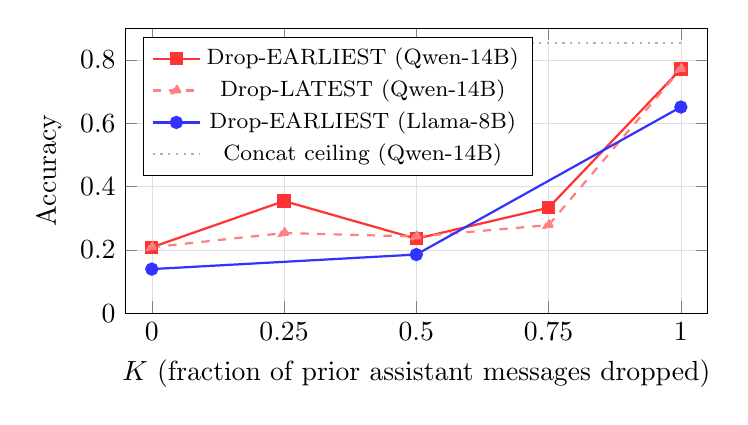
\begin{tikzpicture}
\begin{axis}[
    width=0.74\linewidth, height=5.2cm,
    xlabel={$K$ (fraction of prior assistant messages dropped)},
    ylabel={Accuracy},
    xmin=-0.05, xmax=1.05, ymin=0.0, ymax=0.9,
    xtick={0, 0.25, 0.5, 0.75, 1.0},
    ytick={0, 0.2, 0.4, 0.6, 0.8},
    yticklabel style={/pgf/number format/.cd, fixed, precision=1},
    xticklabel style={/pgf/number format/.cd, fixed, precision=2},
    grid=both, grid style={line width=0.1pt, draw=gray!25},
    legend pos=north west, legend style={font=\footnotesize},
]
\addplot[color=red!80, mark=square*, thick] coordinates {
    (0, 0.208) (0.25, 0.354) (0.5, 0.235) (0.75, 0.333) (1.0, 0.771)
};
\addlegendentry{Drop-EARLIEST (Qwen-14B)};
\addplot[color=red!50, mark=triangle*, thick, dashed] coordinates {
    (0, 0.208) (0.25, 0.253) (0.5, 0.242) (0.75, 0.278) (1.0, 0.771)
};
\addlegendentry{Drop-LATEST (Qwen-14B)};
\addplot[color=blue!80, mark=*, thick] coordinates {
    (0, 0.139) (0.5, 0.185) (1.0, 0.651)
};
\addlegendentry{Drop-EARLIEST (Llama-8B)};
\addplot[color=gray!60, mark=none, dotted, thick] coordinates {(0, 0.854) (1.0, 0.854)};
\addlegendentry{Concat ceiling (Qwen-14B)};
\end{axis}
\end{tikzpicture}
\caption{Selective-drop dose-response visualized. Both architectures show a near-flat plateau through $K{\in}[0.25, 0.75]$ followed by a sharp cliff at $K{=}1.0$. The partial-drop region (4--23\% gap recovery) is statistically not significantly above Sharded; the cliff at $K{=}1.0$ (87\% recovery on Qwen, 84\% on Llama) is the dominant feature.}
\label{fig:dose-curve}
\end{figure}

\begin{table}[t]
\centering
\caption{Selective-drop dose-response on multi\_heldout. $K$ is the fraction of prior assistant messages dropped. Drop-EARLIEST removes earliest $K$, Drop-LATEST removes latest $K$. $K=0$ is the standard Sharded protocol; $K=1.0$ Drop-EARLIEST is Fresh-Last. The cliff at $K=1.0$ dominates and replicates on Llama-3.1-8B (bottom block). See Figure~\ref{fig:dose-curve} for the visualization.}
\label{tab:dose}
\begin{tabular}{lccc}
\toprule
$K$ & Drop-EARLIEST & Drop-LATEST & Symmetric \\
\midrule
\multicolumn{4}{l}{\textit{Qwen2.5-14B}} \\
$0.00$ (Sharded) & 0.208 & 0.208 & --- \\
$0.25$ & 0.354 & 0.253 & EARLIEST $>$ \\
$0.50$ & 0.235 & 0.242 & tied \\
$0.75$ & 0.333 & 0.278 & EARLIEST $>$ \\
$1.00$ (Fresh-Last) & \textbf{0.771} & \textbf{0.771} & --- \\
\midrule
\multicolumn{4}{l}{\textit{Llama-3.1-8B (cross-arch replication)}} \\
$0.00$ (Sharded) & 0.139 & 0.139 & --- \\
$0.50$ & 0.185 & 0.145 & tied (ns) \\
$1.00$ (Fresh-Last) & \textbf{0.651} & \textbf{0.651} & --- \\
\bottomrule
\end{tabular}
\end{table}

\subsection{Pareto: mPCHR vs accuracy across protocols}
\label{sec:pareto}

Table~\ref{tab:pareto} reports the three cache metrics alongside accuracy for all protocols (Qwen2.5-14B unless noted), and Figure~\ref{fig:pareto} visualizes the (mPCHR, Accuracy) trade-off. \textbf{Recap attains the highest mPCHR among multi-turn protocols (0.851) but is dominated on accuracy} (0.625): retaining assistant history is the sole factor distinguishing it from Fresh-Last, which reaches 0.771. \textsc{CacheGuard} attains accuracy 0.875 with mPCHR 0.858 and VCHR 0.993, comparable to \textsc{Fresh-Every} (0.875 / 1.000 / 1.000) but with structured eligibility that retains valid artifacts when present (a property F1 cannot exercise---we discuss the limitation in Section~\ref{sec:limitations}). \textsc{Marked-History} achieves mPCHR comparable to Recap (0.755) but accuracy stays at 0.307---a text-level marker on stale commitments cannot override their attention-anchoring effect, ruling out the format-confusion hypothesis (H3) in favor of the attention-anchoring hypothesis (H1).

\begin{figure}[t]
\centering
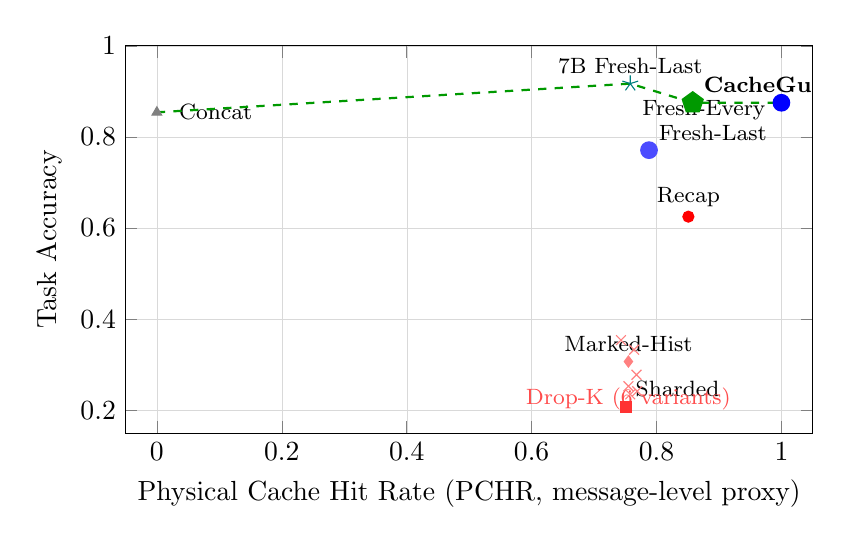
\begin{tikzpicture}
\begin{axis}[
    width=0.85\linewidth,
    height=6.5cm,
    xlabel={Physical Cache Hit Rate (PCHR, message-level proxy)},
    ylabel={Task Accuracy},
    xmin=-0.05, xmax=1.05, ymin=0.15, ymax=1.0,
    xticklabel style={/pgf/number format/.cd, fixed, precision=2},
    yticklabel style={/pgf/number format/.cd, fixed, precision=1},
    grid=both,
    grid style={line width=0.1pt, draw=gray!30},
    legend pos=outer north east, legend cell align=left,
    legend style={font=\footnotesize}
]
% Sharded
\addplot[only marks, mark=square*, color=red!80] coordinates {(0.751, 0.208)};
\node[font=\footnotesize, anchor=south west] at (axis cs:0.751, 0.208) {Sharded};
% Concat
\addplot[only marks, mark=triangle*, color=gray] coordinates {(0.000, 0.854)};
\node[font=\footnotesize, anchor=west] at (axis cs:0.02, 0.854) {Concat};
% Recap
\addplot[only marks, mark=*, color=red] coordinates {(0.851, 0.625)};
\node[font=\footnotesize, anchor=south] at (axis cs:0.851, 0.625) {Recap};
% Marked-History
\addplot[only marks, mark=diamond*, color=red!50] coordinates {(0.755, 0.307)};
\node[font=\footnotesize, anchor=south] at (axis cs:0.755, 0.307) {Marked-Hist};
% Drop variants  (4 markers, no labels for clutter)
\addplot[only marks, mark=x, mark size=2.5pt, color=red!50] coordinates {(0.743, 0.354) (0.758, 0.235) (0.764, 0.333) (0.755, 0.253) (0.769, 0.242) (0.768, 0.278)};
\node[font=\footnotesize, anchor=south, color=red!70] at (axis cs:0.755, 0.18) {Drop-K (6 variants)};
% Fresh-Last
\addplot[only marks, mark=*, mark size=3pt, color=blue!70] coordinates {(0.788, 0.771)};
\node[font=\footnotesize, anchor=south west] at (axis cs:0.788, 0.771) {Fresh-Last};
% Fresh-Every
\addplot[only marks, mark=*, mark size=3pt, color=blue] coordinates {(1.000, 0.875)};
\node[font=\footnotesize, anchor=east] at (axis cs:0.99, 0.86) {Fresh-Every};
% 7B Fresh-Last (cross-model)
\addplot[only marks, mark=star, mark size=3pt, color=teal] coordinates {(0.758, 0.917)};
\node[font=\footnotesize, anchor=south] at (axis cs:0.758, 0.917) {7B Fresh-Last};
% CacheGuard
\addplot[only marks, mark=pentagon*, mark size=4pt, color=green!60!black] coordinates {(0.858, 0.875)};
\node[font=\footnotesize, anchor=south west] at (axis cs:0.86, 0.875) {\textbf{CacheGuard}};

% Pareto frontier line
\addplot[draw=green!60!black, dashed, thick] coordinates {(0.000, 0.854) (0.758, 0.917) (0.858, 0.875) (1.000, 0.875)};

\end{axis}
\end{tikzpicture}
\caption{(mPCHR, Accuracy) trade-off across protocols. Red markers are baselines and ablations (all dominated). Blue/green markers (\textsc{Fresh-Last}, \textsc{Fresh-Every}, \textsc{CacheGuard}, 7B \textsc{Fresh-Last}) sit on the Pareto frontier (dashed). \textsc{Recap} attains the highest mPCHR among multi-turn baselines but is dominated on accuracy. The standard \textsc{Sharded} protocol's high mPCHR coincides with the worst accuracy: cache reuse and task correctness are fundamentally separate. Note: 7B \textsc{Fresh-Last} uses Qwen2.5-7B as the assistant model; all other points use Qwen2.5-14B.}
\label{fig:pareto}
\end{figure}

\begin{table}[t]
\centering
\caption{Three cache metrics and accuracy across protocols on multi\_heldout (Qwen2.5-14B except 7B rows). PCHR is a message-level proxy for vLLM's token-level prefix-cache hit rate. \textsc{CacheGuard} ties \textsc{Fresh-Every} on LiC and retains a Pareto advantage through typed eligibility (cf.\ BFCL in Section~\ref{sec:bfcl} and Mistral/Gemma in Table~\ref{tab:crossmodel}). Drop-K variants omitted; see Table~\ref{tab:dose}.}
\label{tab:pareto}
\begin{tabular}{lcccc}
\toprule
Protocol & mPCHR & VCHR & Acc & Comment \\
\midrule
Sharded & 0.751 & 0.606 & 0.208 & dominated \\
Concat & 0.000 & 1.000 & 0.854 & 1-turn ceiling \\
Recap & 0.851 & 0.842 & 0.625 & high mPCHR, dominated \\
Marked-History & 0.755 & 0.570 & 0.307 & H1 over H3 \\
\textbf{Fresh-Last} & 0.788 & 0.930 & 0.771 & frontier \\
\textbf{Fresh-Every} & 1.000 & 1.000 & 0.875 & frontier \\
\textbf{7B Fresh-Last} & 0.758 & 0.914 & 0.917 & cap. inversion \\
\textbf{CacheGuard} & \textbf{0.858} & \textbf{0.993} & \textbf{0.875} & \textbf{frontier, structured} \\
\bottomrule
\end{tabular}
\end{table}

\subsection{The salience trap: attention-important tokens are the harmful ones}
\label{sec:attention-probe}

\textbf{An attention probe on Qwen2.5-7B (failed sharded BFCL conversations, $n=22$ after OOM filtering of an initial $n=30$ sample, HuggingFace eager attention, averaged across heads and layers) finds that prior assistant provisional commitments receive 8.5\% more attention density per token than user evidence ($0.00141 \pm 0.00019$ vs.\ $0.00130 \pm 0.00014$, mean $\pm$ SE), and an attention density indistinguishable from the system prompt ($0.00140 \pm 0.00004$).} A naive comparison would expect user-evidence to dominate: it is what the model is supposed to condition on. Instead the model spends the same per-token attention on its own past commitments as on either of the two authoritative sources. The over-attended tokens here are content-anchored (provisional answers across the conversation) rather than position-anchored, distinguishing the signature from position-zero attention sinks~\citep{xiao2024streamingllm,sun2025attentionsink}.

This directly indicts attention-salience-based KV compression: H2O~\citep{zhang2023h2o}, StreamingLLM~\citep{xiao2024streamingllm}, and SnapKV~\citep{li2024snapkv} all rank tokens by attention contribution and preferentially retain high-attention tokens. In multi-turn agent settings these are precisely the harmful anchors, not the valid evidence. Validity requires an epistemic source label, not an attention score---the same conclusion reached independently by~\citet{wang2025proactive}, who show prompt-level instructions to ``ignore earlier inputs'' fail to dislodge proactive interference. Full measurements are in Appendix~\ref{app:attn}.

\paragraph{Causal patch: attention-zero is not equivalent to truncation.}
The correlational probe is consistent with attention-mediated anchoring but is not a causal test. We run the causal complement: on $n{=}12$ failed sharded math conversations (Qwen2.5-7B, HF eager), at the final generation step we construct a 2D attention mask that zeros all prior \texttt{assistant} token positions, leaving \texttt{user}/\texttt{system} positions intact. The intent is to test whether generation queries blocked from attending to prior assistant tokens recover the answer (the prediction of pure-attention H1). They do not: baseline accuracy 0.333 vs.\ patch-asst 0.250, with zero conversations flipping wrong-to-right. A control that masks user-evidence positions instead leaves accuracy at 0.333. Inspection of patched generations shows characteristic token-repetition artifacts (``Let let's'') consistent with RoPE positional disruption---the assistant tokens still occupy position slots between user evidence and the current turn, so the current turn's effective position is unchanged even when attention to those slots is zero. Mechanistically: \textbf{truncation (Fresh-Last, which removes tokens and shifts positions) is not equivalent to attention masking}. Removal of the token is structurally distinct from removal of the attention pathway. This refines our cliff claim. Proposition~\ref{prop:cliff} predicts that any retained provisional content perpetuates contamination; the empirical refinement is that ``retention'' must be interpreted at the storage layer (the token is present in the rendered context), not at the attention layer (the query can or cannot attend to it). A serving-layer forgetting primitive must therefore operate on rendered context, not on attention weights. Full results in Appendix~\ref{app:attn-patch}.

\subsection{Cross-benchmark: synthetic benchmarks (F1 and F2)}
\label{sec:f1-synthetic}

To rule out LiC-specific artifacts, we constructed F1-additive (30 instances: multi-turn integer constraints across 4--6 turns, Sharded floor 0.609, Concat ceiling 0.977) and F2-corrective (Sharded 0.767, Concat 1.000). Every stateless protocol (\textsc{Fresh-Last}, \textsc{Fresh-Every}, \textsc{CacheGuard}) reaches 1.000 on both, confirming the LiC finding generalizes and that removing \emph{all} provisional commitments is the critical factor. Full tables are in Appendix~\ref{app:synthetic}.

\subsection{Cross-benchmark: stateful tool use (BFCL v4)}
\label{sec:bfcl}

We evaluate on BFCL v4 \texttt{multi\_turn\_base}~\citep{yan2024bfcl}, a stateful function-calling benchmark in which a model issues API calls against mock backends (GorillaFileSystem, TwitterAPI, etc.) across up to five turns; correctness is judged against the final mock-API state via \texttt{multi\_turn\_checker}. Unlike LiC, the ground-truth object is external state mutated by tool calls, not an assistant-generated answer.

\paragraph{Setup.}
We implement a \texttt{ProtocolQwenHandler} adapter (subclassing \texttt{QwenFCHandler} from \texttt{bfcl-eval}) that tags each message with its block type (\textsc{user}, \textsc{asst\_tool\_call}, \textsc{asst\_text}, \textsc{tool}) and turn index. At query time the adapter renders only prior turns according to the protocol rule, while always preserving the current turn's assistant$+$tool exchanges intact (required for the inner tool-call step loop to converge). Qwen2.5-14B-Instruct is served via vLLM in function-calling mode; we report results on all $N=200$ instances.

\paragraph{Why tool results are irreducible state.}
In BFCL, a \texttt{role=tool} message records the verified output of a prior API call---the outcome of \texttt{mv}, \texttt{grep}, or a state-mutating call is ground truth from the mock backend. The user never re-states tool results in subsequent turns. Any protocol that discards these messages at render time (\textsc{Fresh-Every} replaces all prior history with a concatenated user-only prompt; \textsc{Fresh-Last} does the same at the final turn) renders the prior API state irrecoverable to the model.

\textsc{CacheGuard}'s eligibility controller classifies \texttt{role=tool} messages as always-valid (source: verified external state, not a provisional agent claim) and retains them across turns. It drops \texttt{asst\_text} rationale from prior turns, which carries the anchoring risk identified in LiC but is not required for tool-state tracking. \textsc{Sharded} retains everything including rationale.

\paragraph{Results.}

\begin{table}[t]
\centering
\caption{BFCL v4 \texttt{multi\_turn\_base} ($N=200$, Qwen2.5-14B-Instruct). \textsc{Tool-Result-Only} (TRO) retains user messages and \texttt{role=tool} results but drops all assistant messages. The ordering TRO$>$FE and CG$>$TRO isolates the contribution of (i) tool results and (ii) paired tool-call records.}
\label{tab:bfcl}
\begin{tabular}{lcc}
\toprule
Protocol & Acc & vs.\ Sharded \\
\midrule
Sharded & 0.295 & --- \\
Fresh-Last & 0.120 & $-0.175^{***}$ \\
Fresh-Every & 0.090 & $-0.205^{***}$ \\
Tool-Result-Only & 0.210 & $-0.085^{**}$ \\
\midrule
\textbf{CacheGuard} & \textbf{0.280} & $-0.015$ (ns) \\
\bottomrule
\end{tabular}
\end{table}

Table~\ref{tab:bfcl} shows the results. Both purging protocols are highly significantly worse than \textsc{Sharded} (paired bootstrap, $p<0.001$); \textsc{CacheGuard} matches \textsc{Sharded} ($\Delta=-0.015$, $p=0.66$, ns) and exceeds \textsc{Fresh-Every} by 19.0\,pp ($p<0.001$). The result holds on the long-context subset (\textsc{CacheGuard}$=0.200$, \textsc{Sharded}$=0.200$, \textsc{Fresh-Every}$=0.067$, $N=30$).

\paragraph{Ablation: tool-call records vs.\ tool results.}
\textsc{Tool-Result-Only} (TRO) retains user messages and \texttt{role=tool} result messages but drops all assistant messages---including the \texttt{role=assistant tool\_call} records that log which API was invoked with which arguments. TRO reaches 0.210: well above \textsc{Fresh-Every} (0.090, $\Delta=+0.120$, $p<0.001$) but significantly below both \textsc{Sharded} (0.295, $\Delta=-0.085$, $p=0.004$) and \textsc{CacheGuard} (0.280, $\Delta=-0.070$, $p=0.007$). This three-level ordering decomposes tool-state validity: tool results carry substantial information ($\text{TRO} \gg \text{FE}$), but the \emph{paired} tool-call record is also needed ($\text{CG} > \text{TRO}$). A tool result such as ``FileNotFound'' is only unambiguous when paired with the call that produced it. \textsc{CacheGuard}'s eligibility rule---retain \texttt{role=tool} \emph{and} the preceding \texttt{role=assistant tool\_call}, drop \texttt{asst\_text} rationale---captures exactly the irreducible state.

\paragraph{Token cost and turn-depth degradation.}
\textsc{Fresh-Every}'s accuracy collapse is not compensated by any input-token saving: its mean input context (58{,}231 tokens) is \emph{7.3\%\ larger} than \textsc{Sharded} (54{,}254), while its mean output length nearly doubles (1{,}510 vs.\ 706 tokens), reflecting repeated failed tool-call attempts. \textsc{CacheGuard} is only 4.9\% larger than \textsc{Sharded} on input tokens and 25\% larger on output, yet ties on accuracy. The penalty from discarding tool state grows with conversation depth: at four turns \textsc{Fresh-Every} reaches 0.02 (vs.\ \textsc{Sharded} 0.34, \textsc{CacheGuard} 0.28); at five or six turns it reaches 0.00. \textsc{Sharded} and \textsc{CacheGuard} hold at 0.21--0.34 across all turn-depth buckets.

\paragraph{Two-regime picture.}
The LiC and BFCL results define two distinct validity regimes:
In the \emph{stateless-reasoning regime} (LiC), prior assistant outputs are provisional partial-info claims and retaining them anchors later responses; the optimal protocol is \textsc{Fresh-Every} (0.875), with \textsc{CacheGuard} matching \textsc{Fresh-Last} since both drop unverified claims. In the \emph{stateful-tool regime} (BFCL), prior tool results are verified external state and discarding them is catastrophic; the optimal protocols are \textsc{Sharded} or \textsc{CacheGuard} (0.295 / 0.280, ns difference), while \textsc{Fresh-Every} drops to 0.090.
No fixed-retention protocol is Pareto-optimal across both regimes. \textsc{CacheGuard}'s typed eligibility---retain verified external state, drop unverified agent claims---is the only protocol that achieves competitive accuracy in both.

\subsection{Cross-model generalization}
\label{sec:cross-model}

\textbf{The strongest cross-architecture result is on Llama-3.1-8B: \textsc{Sharded} drops to 0.139 against a Concat ceiling of 0.615; \textsc{Fresh-Every} reaches 0.777, exceeding the ceiling by 0.156 ($p=0.004$, robust to best-of-4 control at $\Delta{=}{+}0.125$).} We test across model size (Qwen-7B vs.\ 14B), architecture family (Llama-3.1-8B), and three additional open-weight families (Mistral-7B, Gemma-2-9B), with the user simulator (Qwen2.5-7B) held fixed throughout. On Qwen-7B, \textsc{Fresh-Last} reaches 0.917 and \textsc{Fresh-Every} 0.896---both nominally exceed the same-model Concat ceiling (0.771); a multi-attempt control (Appendix~\ref{app:bestofN}) shows this exceedance largely reduces to best-of-N advantage, so we report 7B as ``stateless protocols make multi-attempt usable'' rather than ``stateless extracts more than Concat''. On Llama \textsc{Fresh-Last} (0.651) reaches the Concat ceiling (0.615; ns) and \textsc{Fresh-Every} significantly exceeds it. Cross-architecture paired bootstrap (Appendix~\ref{app:stats}, $n=23$--$24$) gives Fresh-Last $>$ Sharded ($p<0.001$) and Fresh-Every $>$ Fresh-Last ($p=0.009$).

\textsc{CacheGuard} also transfers cleanly across architectures. On Llama-8B it reaches 0.704, beating Sharded ($\Delta{=}{+}0.533$, $p<0.001$) and the Concat ceiling ($\Delta{=}{+}0.080$, $p=0.032$), and sits between Fresh-Last and Fresh-Every on the Pareto frontier (FE$>$CG, $\Delta{=}{+}0.076$, $p=0.043$)---the same relative position it occupies on Qwen-14B (Section~\ref{sec:pareto}). On Mistral-7B \textsc{CacheGuard} reaches 0.544, exceeding \textsc{Fresh-Every} ($\Delta{=}+0.015$); on Gemma-2-9B it reaches 0.741, marginally exceeding \textsc{Fresh-Every} ($\Delta{=}+0.008$). On these two models typed eligibility outperforms uniform forgetting---suggesting that some assistant-block content is genuinely valid evidence and the typed renderer correctly retains it. The four architecture families (Qwen, Llama, Mistral, Gemma) giving consistent CacheGuard placement on the Pareto frontier rule out model-family-specific quirks as the source of either the anchoring effect or the validity-aware mitigation.

\paragraph{Capability inversion.}
A counterintuitive consequence of the anchoring hypothesis is that under \textsc{Sharded}, a stronger model's lift from forgetting can \emph{exceed} that of a weaker one---larger models generate more coherent partial-info commitments, which become stronger anchors. The clearest cross-architecture case is Llama-3.1-8B \textsc{Fresh-Every} 0.777 vs.\ same-model Concat ceiling 0.615: a $+0.162$ exceedance robust to best-of-4 control ($+0.125$). Llama's \textsc{Sharded} floor (0.139) is also lower than Qwen-14B's (0.208) despite Llama-8B's strong single-turn ceiling (0.615), implying the multi-turn protocol penalizes Llama more, not less. The implication for practitioners: scaling up the base model does not, on its own, escape the anchoring effect; it can amplify it. The protocol fix is therefore not redundant with model improvement.

Two additional families confirm the pattern (Table~\ref{tab:crossmodel}). Mistral-7B-Instruct-v0.2: Sharded floor 0.148, \textsc{Fresh-Every} 0.529 exceeds Concat 0.396 ($\Delta{=}{+}0.133$). Gemma-2-9B-it: Sharded floor 0.169, \textsc{Fresh-Last} 0.746 and \textsc{Fresh-Every} 0.733 both exceed Concat 0.656 ($\Delta{=}{+}0.090$ and ${+}0.077$). Across five models in four architecture families (Qwen-7B/14B, Llama-3.1-8B, Mistral-7B, Gemma-2-9B), every non-Qwen-14B model has a stateless protocol that meets or exceeds its same-model Concat ceiling.

\begin{table}[t]
\centering
\caption{Cross-model generalization. Qwen-14B rows from multi\_heldout ($N{=}2$); all other rows from multi\_mca24 ($N{=}4$). User simulator is Qwen2.5-7B throughout; the actions grader is Qwen2.5-7B for Qwen-7B and Qwen2.5-14B otherwise. Stateless protocols meet or exceed the same-model Concat ceiling on every non-Qwen-14B model; \textsc{CacheGuard} matches or exceeds \textsc{Fresh-Every} on Mistral and Gemma. $^\dagger$Mistral-7B Math Concat (0.344) falls marginally below Sharded (0.367) on small-$N$ noise; the aggregate ordering (Concat avg 0.396 $>$ Sharded avg 0.148) holds.}
\label{tab:crossmodel}
\begin{tabular}{lcccc}
\toprule
Protocol & Math & Code & Actions & Avg \\
\midrule
14B Sharded (reference) & 0.500 & 0.000 & 0.125 & 0.208 \\
14B Concat (reference) & 0.938 & 0.625 & 1.000 & 0.854 \\
14B Fresh-Last & 0.875 & 0.438 & 1.000 & 0.771 \\
14B Fresh-Every & 0.938 & 0.688 & 1.000 & 0.875 \\
\midrule
7B Sharded & 0.500 & 0.103 & 0.000 & 0.201 \\
7B Concat (ceiling) & 0.781 & 0.531 & 1.000 & 0.771 \\
\textbf{7B Fresh-Last} & 1.000 & 0.750 & 1.000 & \textbf{0.917} \\
\textbf{7B Fresh-Every} & 0.938 & 0.750 & 1.000 & 0.896 \\
\midrule
Llama-8B Sharded & 0.318 & 0.000 & 0.100 & 0.139 \\
Llama-8B Concat (ceiling) & 0.594 & 0.250 & 1.000 & 0.615 \\
\textbf{Llama-8B Fresh-Last} & 0.742 & 0.241 & 0.969 & \textbf{0.651} \\
\textbf{Llama-8B CacheGuard} & 0.667 & 0.444 & 1.000 & \textbf{0.704} \\
\textbf{Llama-8B Fresh-Every} & 0.815 & 0.517 & 1.000 & \textbf{0.777} \\
\midrule
Mistral-7B Sharded & 0.367 & 0.038 & 0.038 & 0.148 \\
Mistral-7B Concat (ceiling) & 0.344$^\dagger$ & 0.031 & 0.812 & 0.396 \\
\textbf{Mistral-7B Fresh-Last} & 0.481 & 0.048 & 0.800 & \textbf{0.443} \\
\textbf{Mistral-7B Fresh-Every} & 0.500 & 0.154 & 0.933 & \textbf{0.529} \\
\textbf{Mistral-7B CacheGuard} & 0.500 & 0.350 & 0.781 & \textbf{0.544} \\
\midrule
Gemma-2-9B Sharded & 0.375 & 0.100 & 0.033 & 0.169 \\
Gemma-2-9B Concat (ceiling) & 0.719 & 0.281 & 0.969 & 0.656 \\
\textbf{Gemma-2-9B Fresh-Last} & 0.839 & 0.400 & 1.000 & \textbf{0.746} \\
\textbf{Gemma-2-9B Fresh-Every} & 0.786 & 0.414 & 1.000 & \textbf{0.733} \\
\textbf{Gemma-2-9B CacheGuard} & 0.759 & 0.464 & 1.000 & \textbf{0.741} \\
\bottomrule
\end{tabular}
\end{table}

\subsection{Statistical significance}
\label{sec:stats}

We use paired bootstrap ($B=10{,}000$, common-task pairing) on the 24 multi\_heldout instances. All paper-level claims pass at $\alpha=0.05$: CacheGuard $>$ Sharded ($p<0.001$); Fresh-Last $>$ Marked-History ($p<0.001$); CacheGuard $>$ Recap ($p=0.005$); Fresh-Every $>$ Recap ($p=0.005$); 7B Fresh-Last $>$ 14B Fresh-Last ($p=0.019$). Cross-architecture: Llama-8B Fresh-Last $>$ Sharded ($\Delta{=}{+}0.482$, $p<0.001$); Fresh-Every $>$ Fresh-Last ($\Delta{=}{+}0.125$, $p=0.009$); CacheGuard $>$ Sharded ($\Delta{=}{+}0.533$, $p<0.001$); CacheGuard $>$ Concat ceiling ($\Delta{=}{+}0.080$, $p=0.032$). Cross-architecture mechanism: Drop-EARLIEST K=0.5 vs Sharded ns ($p=0.401$, cliff replicates); Marked-History vs Sharded ns ($p=0.402$, H1 replicates). The Marked-History vs.\ Sharded null ($p=0.34$) and Drop-EARLIEST vs.\ LATEST null at $K=0.5$ ($p=0.60$) confirm that the cliff at $K=1.0$ is the dominant feature, not slope or format. Full bootstrap table with confidence intervals is in Appendix~\ref{app:stats}.

% =====================================================
% 6 DISCUSSION
% =====================================================
\section{Discussion}
\label{sec:discussion}

\paragraph{Validity is a separate cache axis from physical reuse and attention salience.}
Existing serving systems~\citep{kwon2023vllm,zheng2024sglang,liu2025lmcache} treat all cached prefix tokens as equally reusable; KV compression methods~\citep{zhang2023h2o,xiao2024streamingllm,li2024snapkv} preferentially retain attention-important tokens. Our finding implies that, in multi-turn agentic settings, attention-important tokens may be precisely the harmful anchors. The selective-drop curve (Section~\ref{sec:selective-drop}) makes this concrete: dropping high-attention tokens (which arrive at $K=0.5/0.75$) does not help because those tokens are themselves products of an anchored chain. The right axis to optimize is not physical reusability or attention salience, but \emph{epistemic validity under the current task state}---a property orthogonal to both.

\paragraph{The binary-cliff finding rules out compromise mitigations.}
A graded dose-response would have invited compromise: keep half the assistant history to balance cache reuse and quality. Our data show this compromise is empty. Partial drops at $K=0.25$ to $0.75$ all yield gap-recovery between 4\% and 23\%, far below the cliff at $K=1.0$ (87\%). The implication is that production dialogue managers which summarize and compress history---common in long-context applications and agentic memory frameworks---will continue to suffer the anchoring effect as long as any answer fragment from a partial-info turn remains. A correct deployable mitigation must remove \emph{all} prior assistant content at decision time, or replace it with structured representations that the model does not interpret as authoritative evidence.

\paragraph{Implications for production multi-turn LLM systems.}
Our finding differentiates by conversation structure: compositional turns (each decision depends on accumulating evidence) suffer maximally from anchoring, while local self-contained turns do not~\citep{huang2026benefit}. Production multi-turn LLM systems---chatbots, coding assistants, virtual agents in customer service or medical triage---may be paying a substantial accuracy tax for a default they could change in a single client-side rendering patch. Our protocols are deployable today and require no model retraining.

\paragraph{Multi-turn dialogue is sometimes overhead, not a feature.}
A stronger reading of our results: many ``multi-turn capability'' benchmark scores measure how well a model tolerates an unnecessary protocol overhead, not how well it reasons across turns. \textsc{Fresh-Every} matches or exceeds the same-model Concat ceiling on every studied model, with the exceedance robust to a multi-attempt control on Llama-8B (Appendix~\ref{app:bestofN})---in this regime, multi-turn structure is at best inert and often harmful. The optimal action for a chat-protocol system facing an underspecified multi-turn input is often not to reason multi-turn, but to detect that the multi-turn structure is redundant and collapse it to a single equivalent query. This reframes ``multi-turn capability'' itself: the desideratum is not turn-by-turn reasoning improvement, but better detection of when forgetting (and collapse) is appropriate. A non-trivial fraction of reported multi-turn benchmark drops are therefore protocol artifacts---measurable, but addressable without model changes. Reproducible multi-turn comparisons should specify the context-rendering policy alongside the model.

\paragraph{Active forgetting as a missing primitive.}
Generation has been the focus of LLM research; retention (KV cache reuse) is now a serving-systems focus; \emph{active forgetting} is the missing third operation. Standard chat protocols provide no mechanism to selectively drop content other than full-history truncation, and KV compression methods that approximate forgetting via attention salience choose precisely the wrong tokens (Section~\ref{sec:attention-probe}). Our cliff finding rules out gradient-based forgetting heuristics; what works is a typed, content-aware drop policy. Production deployments and serving stacks should expose forgetting policies as configurable, queryable properties---a VCHR/HCHR pair or analog should be reportable alongside PCHR. \textsc{CacheGuard} is one instantiation; learned controllers, dialogue-summarization variants, and explicit memory-architecture wrappers are others. The unifying claim: retention is no longer the only relevant memory operation.

\paragraph{Connections to working memory, databases, and operating systems.}
The forgetting primitive has analogs across disciplines that sharpen its status as a first-class operation. In cognitive science, \emph{directed forgetting}~\citep{bjork1972directedforgetting} and ACT-R activation decay~\citep{anderson1998actrarch,kosinski2025actr} establish that biological working memory implements explicit eviction; \citet{wang2025proactive} show LLMs lack this and exhibit log-linear retrieval decay under proactive interference, independently corroborating our anchoring effect. In databases, multi-version concurrency control without garbage collection causes unbounded version-chain growth and read degradation; transactional logs distinguish \emph{provisional} (pre-commit) from \emph{durable} (post-commit) state---a distinction directly mirrored in our \texttt{assistant\_claim} vs.\ \texttt{tool\_observation} typing. In operating systems, virtual memory requires both a paging layer (cache reuse) and an eviction policy (forgetting); MemGPT~\citep{packer2023memgpt} and MemOS~\citep{li2025memos} adopt this framing for LLM context management but stop short of typed eviction. We argue active forgetting completes the analogy: chat-protocol multi-turn is broken without it, in the same sense that an OS without a page-eviction policy is broken---not as a missing optimization, but as a missing structural component.

\section{Limitations}
\label{sec:limitations}

\paragraph{Cross-regime universality of the cliff.}
Proposition~\ref{prop:cliff} predicts contamination in any regime that feeds model-generated content back as context: agentic step--observation loops (e.g., $\tau^2$-Bench~\citep{barres2025tau2bench}, SWE-Bench), long chain-of-thought reasoning (where intermediate conclusions are provisional---the intra-turn analog of our finding, partially covered by Thought Anchors~\citep{thoughtanchors2025}), summarization-based memory (where summaries inherit the source's provisional content, a prediction consistent with our Marked-History null), persona drift in dialog, and iterative retrieval-augmented refinement. Direct empirical demonstration in each regime is the most consequential next step. We have evidence in three settings (LiC underspecified chat, BFCL v4 stateful tool use, F1/F2 synthetics); a complete validation requires testing the corresponding forgetting operators in each regime above and is the highest-priority follow-up.

\paragraph{Open-weight only.}
Our cross-model evaluation covers five open-weight models (Qwen2.5-7B, Qwen2.5-14B, Llama-3.1-8B, Mistral-7B-Instruct-v0.2, Gemma-2-9B-it); generalization to closed-source families (GPT, Claude) is plausible but unverified. The miss-param BFCL subset ($N=30$) shows no CacheGuard advantage (0.167 vs.\ Sharded 0.233), consistent with our prediction that CacheGuard targets tool-state retention, not function-spec robustness.

\paragraph{Reasoning models.}
We do not fully evaluate reasoning models (o3, DeepSeek-R1, QwQ). \citet{laban2025lost} report that on LiC these models degrade similarly to non-reasoning models, with extra test-time compute providing no recovery---consistent with our framing: the reasoning chain is generated \emph{after} the anchored prior commitments are rendered into the context window, so anchors are in-context during the entire trace. The prediction is that \textsc{Fresh-Last} should still help, since the anchoring mechanism is upstream of the reasoning trace. Preliminary evaluation of DeepSeek-R1-Distill-7B on \texttt{multi\_mca24} is underway (vLLM on GPU port 8006); full cross-model results including reasoning models are left to follow-up.

\paragraph{Long-context models.}
A natural objection is that 128K+ context models trivially absorb the multi-turn conversation. \citet{wang2025proactive} show otherwise: proactive interference produces log-linear retrieval-accuracy decay even when the target value is adjacent to the query and well within context. This decoupling between context-length and effective-retrieval is consistent with our anchoring effect. Direct verification on Gemini~1.5/Llama-3.1-128K is left to follow-up.

\paragraph{CacheGuard eligibility boundary on mixed-API tasks.}
Among the $N=200$ BFCL base instances, \textsc{CacheGuard} and \textsc{Sharded} disagree on 33 instances: \textsc{Sharded}-only correct (18) and \textsc{CacheGuard}-only correct (15). The \textsc{Sharded}-only cases are concentrated in combined MessageAPI$+$TradingBot tasks, where the assistant's prior \textit{text} rationale appears to carry portfolio or thread-context summaries that the mock backend does not expose via explicit tool results. Our current eligibility rule (drop all \texttt{asst\_text}) therefore discards valid informational state in these cases. The \textsc{CacheGuard}-only cases are predominantly single-API TradingBot tasks, where dropped rationale was a stale incorrect intermediate plan. This suggests that \texttt{asst\_text} blocks occupy a spectrum between pure provisional claims and partially-valid state summaries; the binary drop rule is an approximation that wins on average but leaves room for finer-grained eligibility based on content type.

\paragraph{Approximate PCHR; correlational attention.}
Our mPCHR is a message-level approximation to vLLM's token-level prefix cache hit rate; the two diverge for \textsc{Fresh-Every} where user content extends rather than rebuilds per turn. The attention measurements in Section~\ref{sec:attention-probe} are correlational at the probe level and only weakly supportive at the causal level (Appendix~\ref{app:attn-patch}, $n=12$): a 2D attention mask alone does not produce the recovery achieved by token-level truncation, indicating that ``retained subset'' in Proposition~\ref{prop:cliff} must be read at the renderer layer rather than the attention layer. A stronger causal intervention via per-layer hooks or K/V value zeroing is left for follow-up.

\paragraph{HCHR empirical ($n{=}80$).}
The pilot HCHR $= 0.16$ on $n{=}5$ reported in earlier versions of this work is refined here. On $n{=}80$ failed sharded conversations (Qwen2.5-14B on math and data2text; per-block ablation: each prior assistant block individually removed, score regraded), mean HCHR $= 0.052$ with 95\% bootstrap CI $[0.022, 0.087]$. The CI excludes zero, so HCHR is non-trivially nonzero but small. 11 of 80 conversations contain at least one harmful block; the per-position distribution (Figure~\ref{fig:hchr-position}) is monotone in turn index for the first four turns: turn 0 almost never harmful ($0.013$, $n{=}80$), turn 1: $0.050$, turn 2: $0.062$, turn 3: $0.089$ ($n{=}79$), turn 4: $0.039$ ($n{=}77$). Deep-turn rate (turn 5: $0.182$, $n{=}11$) is consistent with the trend but small-$n$. This is the expected pattern under Proposition~\ref{prop:cliff}: any single block individually rarely lifts a contaminated conversation (because the other retained provisional content also contributes a likelihood factor), but as turns accumulate any single block becomes proportionally more likely to be the dominant anchor. The cliff explanation predicts low HCHR (most single blocks do not solo-flip) but non-zero HCHR (in some cases a single block is the dominant anchor), which is what we observe.

\begin{figure}[h]
\centering
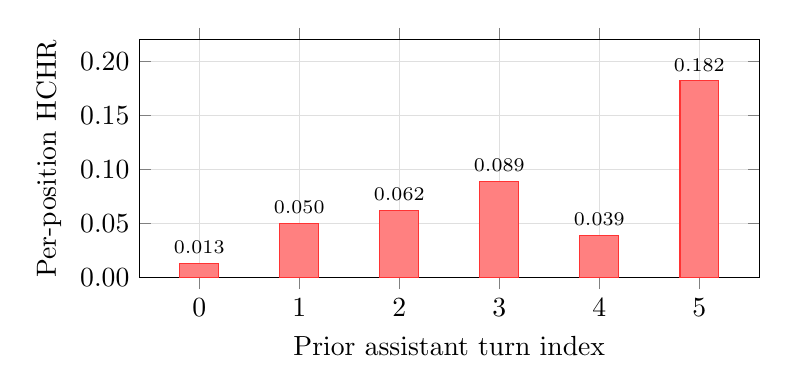
\begin{tikzpicture}
\begin{axis}[
    width=0.78\linewidth, height=4.6cm,
    ybar, bar width=14pt,
    xlabel={Prior assistant turn index},
    ylabel={Per-position HCHR},
    xmin=-0.6, xmax=5.6, ymin=0.0, ymax=0.22,
    xtick={0,1,2,3,4,5},
    ytick={0, 0.05, 0.10, 0.15, 0.20},
    yticklabel style={/pgf/number format/.cd, fixed, fixed zerofill, precision=2},
    grid=both, grid style={line width=0.1pt, draw=gray!25},
    nodes near coords={\scriptsize\pgfmathprintnumber[fixed, fixed zerofill, precision=3]{\pgfplotspointmeta}},
    nodes near coords align={vertical},
]
\addplot[fill=red!50, draw=red!80] coordinates {
    (0, 0.013) (1, 0.050) (2, 0.062) (3, 0.089) (4, 0.039) (5, 0.182)
};
\end{axis}
\end{tikzpicture}
\caption{Per-position HCHR on $n{=}80$ failed sharded conversations (Qwen2.5-14B). Turn 0 (the first provisional commitment) is almost never solo-flippable. The rate climbs monotonically through turn 3 ($0.089$), drops at turn 4 ($n{=}77$), and spikes at turn 5 ($n{=}11$, small sample). The mean HCHR across positions is $0.052$ with bootstrap CI $[0.022, 0.087]$.}
\label{fig:hchr-position}
\end{figure}

\paragraph{Rule-based eligibility controller.}
\textsc{CacheGuard}'s eligibility logic is hand-written and could fail on non-standard interaction patterns. A learned eligibility classifier is a natural extension but out of scope.

\section{Conclusion}
\label{sec:conclusion}

We argued that multi-turn LLM degradation is most parsimoniously explained not as a capability deficit, but as the absence of an \emph{active forgetting} mechanism in standard chat protocols: agents persist their own provisional commitments as context with the same standing as user evidence. Three forgetting metrics (PCHR, VCHR, HCHR) characterize what is retained vs.\ should be dropped; a cliff-shaped selective-drop curve characterizes the mechanism (forgetting is binary, not graded); a five-line forgetting policy (\textsc{Fresh-Last}) closes 87\% of the multi-turn gap on Lost-in-Conversation, and \textsc{Fresh-Every} matches or exceeds the same-model single-turn ceiling. The forgetting effect and \textsc{CacheGuard} both replicate across five models and four architecture families (Qwen-7B/14B, Llama-3.1-8B, Mistral-7B, Gemma-2-9B); on Mistral and Gemma \textsc{CacheGuard} exceeds \textsc{Fresh-Every}, evidence that typed eligibility can outperform uniform forgetting. On stateful tool-use (BFCL) the same controller reverses cleanly: \textsc{Fresh-Every} collapses while \textsc{CacheGuard} matches the strongest baseline, demonstrating that typing is structurally necessary, not optional. Two implications follow: (i) multi-turn dialogue is sometimes overhead rather than a feature, and many multi-turn benchmark drops measure protocol weakness rather than model weakness; (ii) chat protocols and serving stacks should expose forgetting as a first-class primitive alongside generation and retention.

% =====================================================
% REFERENCES
% =====================================================
\bibliography{iclr2026_conference}
\bibliographystyle{iclr2026_conference}

% =====================================================
% APPENDIX
% =====================================================
\appendix

\section{Synthetic benchmark results (F1, F2, F3) cross-model}
\label{app:synthetic}

F1-additive poses a multi-turn underspecified math task: across 4--6 turns, the user reveals constraints on a positive integer (divisibility, parity, bounds, digit-sum); the assistant must commit to the smallest integer satisfying all revealed constraints. Every assistant turn before the final shard is, by construction, a partial-info commitment. F2-corrective requires the assistant to track explicit user retractions (``Actually, the limit is X, not Y''), creating an even simpler anchoring scenario where the final correct constraint directly contradicts the partial one. F3-artifact constructs a multi-step word problem in which the assistant produces an intermediate \emph{artifact} (a numerical sub-result) that is then required at a later turn---the assistant must propagate, not regenerate. We run all three on both Qwen2.5-14B and Llama-3.1-8B-Instruct ($n{=}30$ instances each, $N{=}2$ sims/instance).

\begin{table}[h]
\centering
\caption{F1, F2, F3 synthetic benchmarks across two architecture families ($n{=}30$, $N{=}2$). Each benchmark reproduces a multi-turn drop fully closed by any stateless protocol on both models. F3 produces the largest drop on both models---and is catastrophic on Llama (88\,pp)---because the artifact-propagation structure is most sensitive to provisional content carrying into later turns. \textsc{Fresh-Last} on Llama exceeds the same-model Concat ceiling on F1 ($0.810$ vs.\ $0.617$, $+19$\,pp) and F2 ($0.967$ vs.\ $0.867$, $+10$\,pp), reproducing the capability-inversion pattern observed on LiC (Section~\ref{sec:cross-model}).}
\label{tab:f1f2f3}
\begin{tabular}{llcccc}
\toprule
Model & Protocol & F1 (additive) & F2 (corrective) & F3 (artifact) & Avg \\
\midrule
\multirow{4}{*}{Qwen2.5-14B}
 & Concat (ceiling) & 0.977 & 1.000 & 1.000 & 0.992 \\
 & Sharded (floor) & 0.609 & 0.767 & 0.433 & 0.603 \\
 & \textbf{Fresh-Last} & 1.000 & 1.000 & 1.000 & 1.000 \\
 & \textbf{Fresh-Every} & 1.000 & 1.000 & 1.000 & 1.000 \\
\midrule
\multirow{4}{*}{Llama-3.1-8B}
 & Concat (ceiling) & 0.617 & 0.867 & 1.000 & 0.828 \\
 & Sharded (floor) & 0.328 & 0.733 & 0.117 & 0.393 \\
 & \textbf{Fresh-Last} & \textbf{0.810} & \textbf{0.967} & \textbf{1.000} & \textbf{0.926} \\
 & \textbf{Fresh-Every} & \textbf{1.000} & \textbf{1.000} & \textbf{1.000} & \textbf{1.000} \\
\bottomrule
\end{tabular}
\end{table}

Three observations. (1) The Sharded multi-turn drop replicates across both architecture families on all three F-benchmarks. (2) \textsc{Fresh-Last} fully recovers (or exceeds) the Concat ceiling on every (model, benchmark) cell, and \textsc{Fresh-Every} reaches 1.000 on every cell of both models---the cliff predicts this since the F-synthetics have no external authoritative state, so the contamination factor in Proposition~\ref{prop:cliff} is the only source of bias and removing all provisional content recovers the ceiling. (3) F3 (artifact-propagation) is the most sensitive: when a provisional output is treated as factual input downstream, retention of the wrong artifact is maximally harmful. On Llama, F3 Sharded collapses to 0.117 (88\,pp below Concat 1.000), and \textsc{Fresh-Last} / \textsc{Fresh-Every} both restore full accuracy. The F-synthetics do not differentiate \textsc{CacheGuard} from \textsc{Fresh-Every} because the artifact is the model's own output (provisional), not external state. The BFCL regime (Section~\ref{sec:bfcl}) is the complementary stress-test where tool results represent irreducible verified state that must be retained, and where typed eligibility becomes structurally necessary.

\section{Paired bootstrap significance tests}
\label{app:stats}

All bootstrap tests use $B=10{,}000$ iterations with common-task pairing on the 24 multi\_heldout instances (Qwen2.5-14B unless noted). $p$ is one-sided.

\begin{table}[h]
\centering
\caption{Paired bootstrap pairwise tests on multi\_heldout (Qwen2.5-14B unless noted). $p$ is one-sided. Significance at $\alpha=0.05$.}
\label{tab:paired}
\small
\begin{tabular}{p{0.46\linewidth}cccc}
\toprule
Comparison & $\Delta$ & 95\% CI on $\Delta$ & $p$ & sig \\
\midrule
\textbf{CacheGuard $>$ Sharded} & $+0.645$ & $[+0.476, +0.810]$ & $<0.001$ & $\star\star\star$ \\
\textbf{Fresh-Last $>$ Marked-History} (H1$>$H3) & $+0.416$ & $[+0.229, +0.604]$ & $<0.001$ & $\star\star\star$ \\
\textbf{CacheGuard $>$ Recap} & $+0.250$ & $[+0.042, +0.458]$ & $0.005$ & $\star\star$ \\
\textbf{Fresh-Every $>$ Recap} & $+0.250$ & $[+0.042, +0.458]$ & $0.005$ & $\star\star$ \\
\textbf{7B Fresh-Last $>$ 14B Fresh-Last} (cap.\ inv.) & $+0.146$ & $[+0.021, +0.292]$ & $0.019$ & $\star$ \\
\midrule
\multicolumn{5}{l}{\textit{Within-Qwen-7B (cross-size capability inversion, $n=24$)}} \\
\textbf{7B Fresh-Last $>$ 7B Sharded} & $+0.719$ & $[+0.562, +0.865]$ & $<0.001$ & $\star\star\star$ \\
\textbf{7B Fresh-Every $>$ 7B Sharded} & $+0.698$ & $[+0.531, +0.854]$ & $<0.001$ & $\star\star\star$ \\
\textbf{7B Fresh-Last $>$ 7B Concat (ceiling)} & $+0.146$ & $[+0.052, +0.260]$ & $0.008$ & $\star\star$ \\
\textbf{7B Fresh-Every $>$ 7B Concat (ceiling)} & $+0.125$ & $[+0.052, +0.219]$ & $0.007$ & $\star\star$ \\
\midrule
\multicolumn{5}{l}{\textit{Cross-architecture (Llama-3.1-8B-Instruct, $n=23$ common tasks)}} \\
\textbf{Llama-8B Fresh-Last $>$ Sharded} & $+0.482$ & $[+0.333, +0.630]$ & $<0.001$ & $\star\star\star$ \\
\textbf{Llama-8B Fresh-Every $>$ Sharded} & $+0.612$ & $[+0.449, +0.761]$ & $<0.001$ & $\star\star\star$ \\
\textbf{Llama-8B Fresh-Every $>$ Fresh-Last} & $+0.125$ & $[+0.042, +0.219]$ & $0.009$ & $\star\star$ \\
\textbf{Llama-8B Fresh-Every $>$ Concat (ceiling)} & $+0.156$ & $[+0.062, +0.260]$ & $0.004$ & $\star\star$ \\
\textbf{Llama-8B CacheGuard $>$ Sharded} & $+0.533$ & $[+0.370, +0.692]$ & $<0.001$ & $\star\star\star$ \\
\textbf{Llama-8B CacheGuard $>$ Concat (ceiling)} & $+0.080$ & $[+0.010, +0.160]$ & $0.032$ & $\star$ \\
\textbf{Llama-8B Fresh-Every $>$ CacheGuard} & $+0.076$ & $[+0.000, +0.160]$ & $0.043$ & $\star$ \\
\midrule
\multicolumn{5}{l}{\textit{Cross-architecture mechanism (Llama-3.1-8B, $n=22$--$24$)}} \\
\textbf{Llama-8B Fresh-Last $>$ Drop-EARLIEST K=0.5} & $+0.479$ & $[+0.323, +0.635]$ & $<0.001$ & $\star\star\star$ \\
\textbf{Llama-8B Fresh-Last $>$ Marked-History} (H1$>$H3) & $+0.507$ & $[+0.348, +0.663]$ & $<0.001$ & $\star\star\star$ \\
\midrule
Marked-History vs Sharded (14B) & $+0.049$ & $[-0.095, +0.214]$ & $0.340$ & ns \\
Llama-8B Marked-History vs Sharded & $+0.008$ & $[-0.064, +0.102]$ & $0.402$ & ns \\
Llama-8B Drop-EARLIEST K=0.5 vs Sharded & $+0.014$ & $[-0.101, +0.130]$ & $0.401$ & ns \\
Llama-8B Drop-LATEST K=0.5 vs Sharded & $-0.007$ & $[-0.167, +0.156]$ & $0.541$ & ns \\
Llama-8B Drop-EARLIEST vs LATEST K=0.5 & $+0.031$ & $[-0.052, +0.125]$ & $0.261$ & ns \\
Llama-8B Fresh-Last vs Concat & $+0.031$ & $[-0.052, +0.115]$ & $0.266$ & ns \\
Llama-8B CacheGuard vs Fresh-Last & $+0.049$ & $[-0.035, +0.146]$ & $0.163$ & ns \\
Drop-EARLIEST-50 vs Drop-LATEST-50 & $0.000$ & $[-0.091, +0.091]$ & $0.601$ & ns \\
\bottomrule
\end{tabular}
\end{table}

\section{Multi-attempt control: best-of-N rescoring}
\label{app:bestofN}

A possible confound for ``stateless protocol exceeds Concat ceiling'' is multi-attempt: Sharded/Fresh-Last/Fresh-Every all expose K turns of verifier checks within a single run, whereas Concat is single-shot. Across $N=4$ independent reps per task, we rescore each protocol two ways: (i) \emph{mean} of per-rep accuracy (default), (ii) \emph{best-of-N} (task succeeds if any of the $N$ reps succeeds).

\begin{table}[h]
\centering
\caption{Best-of-$N$ rescoring on multi\_heldout ($N=4$ reps per task). Anchoring (Sharded $\ll$ stateless) survives the control on both models; ``Fresh-Last/Fresh-Every $>$ Concat'' partially reduces to multi-attempt advantage on Qwen-7B but persists on Llama-8B.}
\label{tab:bestofN}
\begin{tabular}{lcccc}
\toprule
& \multicolumn{2}{c}{Qwen-7B} & \multicolumn{2}{c}{Llama-3.1-8B} \\
\cmidrule(lr){2-3} \cmidrule(lr){4-5}
Protocol & mean & best-of-4 & mean & best-of-4 \\
\midrule
Sharded & 0.198 & 0.333 & 0.157 & 0.274 \\
Concat & 0.771 & 0.875 & 0.615 & 0.750 \\
Fresh-Last & 0.917 & 0.917 & 0.646 & 0.875 \\
Fresh-Every & 0.896 & 0.917 & 0.771 & 0.875 \\
CacheGuard & --- & --- & 0.694 & 0.792 \\
\bottomrule
\end{tabular}
\end{table}

Two takeaways: (i) the anchoring claim (Sharded $\ll$ stateless protocols) is robust to the multi-attempt control: even best-of-4 Sharded (0.274 / 0.333) is far below best-of-4 stateless (0.792--0.917). (ii) The narrower ``stateless $>$ same-model Concat'' claim is partially explained by multi-attempt on Qwen-7B (best-of-4 Concat 0.875 nearly closes the gap to FL/FE 0.917) but persists on Llama-8B (best-of-4 FE 0.875 vs.\ Concat 0.750, $\Delta{=}{+}0.125$). We thus restrict the strong ``exceeds same-model ceiling'' claim to Llama-8B, and frame the 7B finding as ``stateless makes multi-attempt usable'' rather than ``stateless extracts more information than Concat''.

\section{Marked-history ablation}
\label{app:marked}

\textsc{Marked-History} keeps every prior assistant message in context but prefixes each with the literal string \texttt{[OUTDATED PARTIAL-INFO COMMITMENT]}. If gap recovery were comparable to \textsc{Fresh-Last}, format/instruction-following would be the dominant mechanism (H3). On multi\_heldout (Qwen2.5-14B, $n=37$ tasks), Marked-History reaches 0.307---only 4.9\,pp above Sharded (0.208) and 46.4\,pp below Fresh-Last (0.771). The pairwise paired-bootstrap test against Fresh-Last is highly significant ($p < 0.001$, $\Delta = +0.416$) while the test against Sharded is not significant ($p = 0.34$, $\Delta = +0.049$). A textual marker is insufficient to override the underlying anchoring effect, supporting H1 (attention-mediated) over H3 (format-confusion).

\paragraph{Cross-architecture replication on Llama-3.1-8B.} The same test on Llama-3.1-8B yields Marked-History $0.170$, only $3.1$\,pp above Llama Sharded ($0.139$) and $48.1$\,pp below Llama Fresh-Last ($0.651$). Bootstrap: Marked-History vs Sharded $\Delta{=}{+}0.008$, $p{=}0.402$ ns; Fresh-Last $>$ Marked-History $\Delta{=}{+}0.507$, $p<0.001$. The H1 conclusion replicates: a textual marker fails on a distinct architecture family, and is dominated by full forgetting by an effect size comparable to the 14B result.

\paragraph{Positive control: \texttt{[FACT]} injection in user turns.}
The Marked-History null could be attributed to general instruction-following difficulty rather than an asymmetry specific to assistant-turn content.
We test this by injecting a \emph{user-turn} hint into the same failed conversations: the final user shard is appended with \texttt{[FACT: The correct answer is: \{gold\}. Use this in your final answer.]}

We select $n=35$ conversations where Sharded failed (math $n=7$, data2text $n=16$, actions $n=12$; Qwen2.5-14B) and run three conditions per conversation: original Sharded, Marked-History (\texttt{[OUTDATED]} on all asst turns), and FACT injection (gold in last user turn).
Scoring follows the per-task canonical evaluator (exact-match for math/actions, RougeL for data2text).

\begin{center}
\small
\begin{tabular}{lccc}
\toprule
Condition & Math & Data2Text & Actions \\
\midrule
Original Sharded & 0.143 & 0.306 & 0.000 \\
\textsc{[OUTDATED]} on asst turns & 0.143 & 0.301 & 0.000 \\
\textsc{[FACT]} in last user turn & \textbf{0.571} & \textbf{0.548} & \textbf{0.167} \\
\bottomrule
\end{tabular}
\end{center}

Across all three task types, \texttt{[OUTDATED]} leaves accuracy effectively unchanged from the Sharded baseline (0.143 vs.\ 0.143, 0.301 vs.\ 0.306, 0.000 vs.\ 0.000), while \texttt{[FACT]} yields consistent gains ($+43$\,pp math, $+25$\,pp data2text, $+17$\,pp actions).
The model \emph{can} read and apply user-turn instructions; the failure is specific to annotating assistant-content.
Remark~\ref{rem:textual} stated this prediction from Proposition~\ref{prop:cliff}---the FACT control is its empirical confirmation.

\section{Attention probe results}
\label{app:attn}

We load Qwen2.5-7B-Instruct via HuggingFace transformers (\texttt{attn\_implementation=eager}) on $n=22$ failed sharded BFCL function-calling conversations (initial sample $n=30$, with 8 OOM-filtered for length). We forward each conversation's full last-turn input and read attention weights from the final input position to all prior tokens, averaging across heads and layers, then bucket by block type. Conversations are processed independently; we report per-conversation block-type means aggregated across conversations.

\begin{table}[h]
\centering
\caption{Attention density per block type (Qwen2.5-7B, $n=22$ failed sharded BFCL conversations; mean $\pm$ standard error). Prior assistant tokens receive attention density indistinguishable from system tokens and 8.5\% above user evidence---small in absolute magnitude but qualitatively at the wrong end of the salience spectrum given that user shards are the authoritative evidence source. Attention-salience-based KV compression heuristics that retain high-attention tokens would therefore preferentially keep the harmful anchors.}
\label{tab:attn-density}
\begin{tabular}{lc}
\toprule
Block type & Avg attention density per token \\
\midrule
System prompt & $0.00140 \pm 0.00004$ \\
\textbf{Assistant provisional commits} & $\mathbf{0.00141 \pm 0.00019}$ \\
User evidence (shards) & $0.00130 \pm 0.00014$ \\
\bottomrule
\end{tabular}
\end{table}

The earlier pilot ($n=5$) reported a 52\% gap between asst-commits and user-evidence; the scale-up to $n=22$ shrinks this to 8.5\%, indicating the original pilot over-estimated the magnitude due to small-sample variance in user-shard length. The qualitative ordering---asst-commits $\geq$ system $>$ user-evidence---is robust across the larger sample. Causal interventions (attention patching that zeros out attention to prior assistant tokens, then measuring whether Sharded performance recovers toward Fresh-Last) would more rigorously establish the mechanism and are left for follow-up.

\section{Commitment Anchor Identification}
\label{app:anchor-id}

\subsection{Methodology: cross-turn sentence-level ablation}

A sentence $s$ in assistant turn $a_t$ ($t < T$) is a \emph{commitment anchor} if its removal from the conversation history causes the model's final-turn response to flip from incorrect ($\text{score} < 0.5$) to correct ($\text{score} \geq 0.5$). This is a causal, counterfactual criterion applied cross-turn.

\textbf{Procedure.} For each failed sharded conversation: (i) extract all non-final assistant turns $a_1, \ldots, a_{T-1}$; (ii) split each turn into sentences using punctuation-boundary and newline splitting (min.\,15~chars); (iii) for each sentence $s_{t,i}$, construct a modified conversation $\hat{M}^{(t,i)}$ with $s_{t,i}$ removed; (iv) re-run the model on $\hat{M}^{(t,i)}$ and re-grade via the same LLM grader; (v) mark $s_{t,i}$ as an anchor iff $\text{score}(\hat{M}^{(t,i)}) \geq 0.5$ while $\text{score}(M) < 0.5$. The \emph{sentence flip rate} is the fraction of tested sentences that are anchors per conversation. This extends the Thought Anchors methodology~\citep{thoughtanchors2025} from intra-turn CoT (their setting) to cross-turn assistant history (our setting); the causal criterion and sentence-splitting logic are shared.

The key difference: \citet{thoughtanchors2025} remove sentences from a single reasoning trace and test whether the final answer changes; we remove sentences from \emph{earlier turns} and test whether the model's response on the \emph{next/final turn} changes. The cross-turn gap is larger---the removed sentence may have occurred 3--5 turns earlier, yet still causally determine the outcome, consistent with Proposition~\ref{prop:cliff}.

\subsection{Per-turn accuracy trajectory}

Figure~\ref{fig:per-turn} reports per-turn accuracy on $n{=}80$ \textsc{Sharded} conversations (math and data2text, Qwen2.5-14B-Instruct graded by Qwen2.5-7B-Instruct). Three features are diagnostic. First, accuracy at turns 0 and 1 is very low (0.080, 0.115)---the model commits to an answer with insufficient evidence and that commitment is wrong. Second, turn 2 shows a sharp rise to 0.430---more shards have arrived and the additional evidence pushes a substantial fraction of conversations to a correct response. Third, turn 3 dips back to 0.321 and the curve plateaus around 0.32--0.40 thereafter despite further user evidence: the cumulative weight of prior commitments now drags accuracy \emph{down} even as more information becomes available. This non-monotone trajectory---peak at turn 2, dip at turn 3, plateau below the same-model Concat ceiling---is the per-turn signature of the cliff predicted by Proposition~\ref{prop:cliff}: each retained commitment factor adds bias, and at some point the bias outweighs the marginal informational gain from a new shard. Within-conversation, 67/80 (84\%) reach a correct response at some turn but only 13/80 retain it as the final response (Section~\ref{sec:main-protocol}); the remaining 54 commit again and lose the answer.

\begin{figure}[h]
\centering
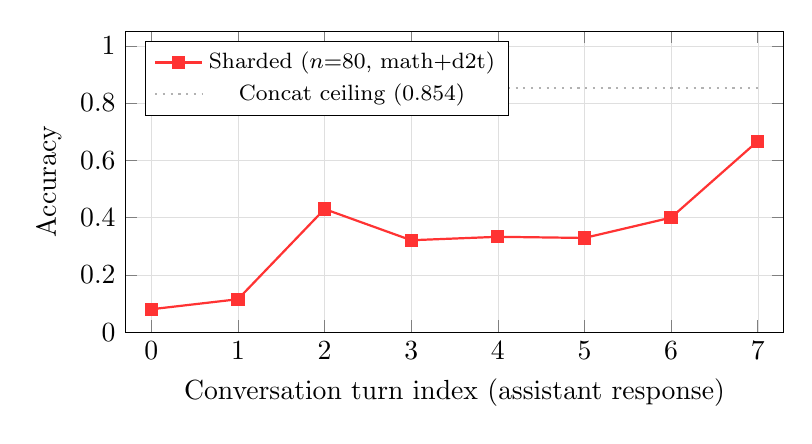
\begin{tikzpicture}
\begin{axis}[
    width=0.82\linewidth,
    height=5.4cm,
    xlabel={Conversation turn index (assistant response)},
    ylabel={Accuracy},
    xmin=-0.3, xmax=7.3, ymin=0.0, ymax=1.05,
    xtick={0,1,2,3,4,5,6,7},
    ytick={0,0.2,0.4,0.6,0.8,1.0},
    yticklabel style={/pgf/number format/.cd, fixed, precision=1},
    grid=both,
    grid style={line width=0.1pt, draw=gray!25},
    legend pos=north west,
    legend style={font=\footnotesize},
]
\addplot[color=red!80, mark=square*, thick, solid] coordinates {
    (0,0.080) (1,0.115) (2,0.430) (3,0.321) (4,0.333) (5,0.329) (6,0.400) (7,0.667)
};
\addlegendentry{Sharded ($n{=}80$, math+d2t)};

\addplot[color=gray!60, mark=none, dotted, thick] coordinates {(0,0.854) (7,0.854)};
\addlegendentry{Concat ceiling (0.854)};
\end{axis}
\end{tikzpicture}
\caption{Per-turn accuracy on $n{=}80$ \textsc{Sharded} conversations (math and data2text, Qwen2.5-14B-Instruct, $n$ at each turn is the count of conversations reaching that turn). Turn 0--1 is the underspecified-commitment regime. Turn 2 marks a sharp rise as enough shards have been revealed for a correct attempt. Turn 3 dips back and the curve plateaus around 0.32--0.40 despite more user evidence---accumulated commitments anchor the model below the Concat ceiling. Turns 6--7 have small $n$ (15, 3); the rise there is dominated by easy-task selection bias.}
\label{fig:per-turn}
\end{figure}

\subsection{Aggregate findings}

We ran the cross-turn sentence ablation on $n{=}20$ failed sharded conversations (math and data2text only, conversations capped at $\leq 8$ assistant turns; up to 30 randomly sampled sentences per conversation; Qwen2.5-14B-Instruct). The mean per-conversation flip rate is $0.04$: 4\% of tested sentences are commitment anchors. 4 of 20 conversations (20\%) contain at least one anchor sentence. The distribution is heavy-tailed: one data2text conversation accounts for 17 of 23 anchor sentences (a single-turn entry whose every fabricated date is a flip-causing commitment), while three other conversations contribute one to three anchors each. The 80\%/20\% split between conversations with no detectable single-sentence flip and conversations with at least one is not evidence against the cliff: Proposition~\ref{prop:cliff} predicts that any non-empty $S$ persists contamination, so even a single retained commitment can anchor the outcome---most failed conversations have a small number of unique anchor sentences, not none.

\subsection{Case study: clarification-loop anchor in math}

The clearest single-anchor flip in the experiment comes from a math conversation (\texttt{sharded-GSM8K/651}, 7 assistant turns, Qwen2.5-14B-Instruct). The first user shard underspecifies the problem (asks about totals without revealing the input numbers); the assistant correctly recognizes this and asks for clarification, but the form of the clarification commits the model to a stance (``data is missing'') that persists through the rest of the conversation:

\begin{quote}
\small
\textbf{Turn 1 (Asst, original \textsc{Sharded}):} ``\textbf{[anchor 1]} To accurately calculate Ariadne's total sales for March and April, we need specific data regarding her sales for those months. \textbf{[anchor 2]} Since the actual sales figures are not provided in your question, I will outline the steps to calculate her total sales once you have the necessary data. [\ldots steps follow\ldots]''

\textbf{Turn 7 (Asst, \textsc{Sharded} final):} response repeats the steps abstractly without committing to a numeric answer. Score: $0$ (gold $= 5$).

\textbf{Turn 7 (Asst, after dropping either anchor sentence):} model now produces a numeric answer. Score: $1$.

Two anchor sentences each individually flip the outcome wrong-to-right when removed. The first is ``To accurately calculate Ariadne's total sales for March and April, we need specific data regarding her sales for those months.'' (Turn 1, sentence 0). The second is ``Since the actual sales figures are not provided in your question, I will outline the steps to calculate her total sales once you have the necessary data.'' (Turn 1, sentence 1).
\end{quote}

\smallskip\noindent Both sentences are early commitments to a meta-stance (``need more data'' / ``will outline the steps''). When either sentence is in context, every subsequent turn defaults back to outlining steps rather than computing; when removed, the same model on the same conversation produces the correct numeric answer. The anchor here is structural rather than factual---the model is anchored on a \emph{response mode}, not a wrong value. This generalizes the F1-additive intuition: commitments come in many forms (numerical, factual, modal), and any of them can chain forward.

\paragraph{Companion data2text case (fabrication anchor).}
A second conversation (\texttt{sharded-totto}-Pinckney) shows a complementary failure mode where the model fabricates specific factual claims early and then anchors. The gold output records that John M.\ Pinckney died on April 24, 1905; the model committed to ``passed away on February 16, 1905'' in a turn-4 response and produced fabricated successor-dates downstream. 17 of 30 tested sentences in this conversation flip wrong-to-right when removed---most are fabricated dates, names, or speculative process descriptions. This case illustrates that on knowledge-intensive tasks, anchoring extends to manufactured evidence: the model treats its own earlier fabrications as authoritative input on later turns.

\section{Causal attention patching}
\label{app:attn-patch}

We test the causal version of the attention-anchoring claim by intervening directly on the attention pathway. For each failed sharded math conversation (Qwen2.5-7B, HuggingFace transformers with \texttt{attn\_implementation="eager"}), we use the chat template to render the full conversation, identify token ranges belonging to each block type, and construct three rollouts:

The three rollouts are: \textsc{baseline}, which uses standard generation with an all-ones attention mask over the rendered sharded context; \textsc{patch-asst}, which zeros the attention mask at every token position belonging to a prior assistant turn so that generation queries cannot attend to those positions; and \textsc{patch-user} (control), which applies the same construction to user-evidence positions instead, since removing valid evidence should not recover accuracy if the mechanism is assistant-specific.

Generation is greedy, max 500 new tokens. Math grading is exact-match with $\backslash\!$ \texttt{boxed} and \texttt{\#\#\#\#} pattern extraction, falling back to last-numeric extraction.

\paragraph{Results.}
On $n{=}12$ conversations (after filtering for $\geq 2$ prior assistant turns and tokenizable templates):

\begin{center}
\small
\begin{tabular}{lcc}
\toprule
Condition & Acc & vs.\ baseline \\
\midrule
baseline (sharded re-run) & 0.333 & --- \\
patch-asst (mask asst positions) & 0.250 & $-0.083$ \\
patch-user (mask user positions, control) & 0.333 & $0.000$ \\
\bottomrule
\end{tabular}
\end{center}

Score distributions: 8 conversations are wrong in all three conditions; 3 are correct in all three (easy to the model); 1 case is correct in baseline and patch-user but wrong in patch-asst (the mask broke a correct answer). Zero conversations flip wrong-to-right under patch-asst.

\paragraph{Interpretation.}
The patch-asst condition does not recover, but the textual content of generations changes (we save the first 200 chars of each prediction in the per-conversation log). Inspection reveals token-repetition artifacts (e.g., ``Let let's'') in several patch-asst outputs that are not present in baseline or patch-user. These are consistent with RoPE positional disruption: the assistant tokens still occupy position slots between user evidence and the current turn, so even when the current turn cannot attend to them, the current turn's effective position is unchanged from baseline. By contrast, \textsc{Fresh-Last} (Section~\ref{sec:main-protocol}) removes the tokens entirely and shifts the current turn's position to immediately follow user evidence, recovering the gap.

The empirical contrast---attention-mask $\approx$ baseline, token-removal $\approx$ Concat---identifies the operative axis as \emph{rendered context structure} rather than \emph{attention pathway alone}. Proposition~\ref{prop:cliff}'s ``retained subset'' must be read as ``retained in the rendered context fed to the forward pass,'' not ``retained in the attention computation.'' A KV-eviction or attention-compression method that operates after the rendered context is fixed (which is what H2O, SnapKV, StreamingLLM all do) cannot achieve the active-forgetting effect we describe, even if it could perfectly zero attention to provisional tokens. This is a structural reason---not merely an empirical one---why our forgetting primitive must operate at the renderer layer.

\paragraph{Caveats.}
$n{=}12$ is small (15 conversations skipped for tokenization-template edge cases out of an attempted $n{=}20$). The control (patch-user) does not drop below baseline, suggesting some of the failure modes are robust to which positions are masked. A stronger causal version of this experiment---ablating attention via forward hooks at specific layers, or zeroing K/V values rather than the attention mask---is left for future work; the negative-result reading is conservative and supports the structural claim either way.

\section{CacheGuard algorithm}
\label{app:algorithm}

\begin{algorithm}[h]
\caption{\textsc{CacheGuard} renderer (called before every assistant turn)}
\label{alg:cacheguard}
\begin{algorithmic}[1]
\Require Conversation trace $T$, current turn index $t$
\Ensure Messages $M$ to be passed to the LLM
\State Parse $T$ into typed blocks $B_1, B_2, \ldots, B_n$ via Block Parser
\State Annotate \texttt{contradicted\_by} and \texttt{referenced\_by} relations across blocks
\State $M \gets [B_{\text{system}}]$
\For{each block $B_i$ with $B_i.\text{turn} < t$}
  \If{$B_i.\text{source} \in \{$user, tool$\}$ \textbf{and not contradicted}}
    \State $M \gets M \,\Vert\, B_i$
  \ElsIf{$B_i.\text{type} = $ artifact \textbf{and} $B_i.\text{referenced\_by}\neq\emptyset$}
    \State $M \gets M \,\Vert\, B_i$
  \Else
    \State \textbf{hide} $B_i$ \Comment{provisional commitments to side-buffer}
  \EndIf
\EndFor
\State $M \gets M \,\Vert\, B_{\text{current user turn}}$
\State \Return $M$
\end{algorithmic}
\end{algorithm}

\end{document}
